\documentclass[12pt, a4paper]{report}
\usepackage[english,italian]{babel}
\usepackage{booktabs}
\usepackage{listings}
\usepackage[utf8]{inputenc}
\usepackage{amsmath}
\usepackage[pdftex]{graphicx}
\usepackage{float}
\usepackage{eurosym}
\usepackage{hyperref}
\usepackage[scientific-notation=true]{siunitx}
\usepackage{wrapfig}
\usepackage{subfig}
\usepackage{cite}
\usepackage{capt-of}
\usepackage{booktabs, caption, makecell}
\renewcommand\theadfont{\bfseries}
\usepackage{threeparttable}
\usepackage{varwidth}
\usepackage{tabularx}


\graphicspath{{./Figure/} {./Figure/Grafici_Finali/}}
\bibliographystyle{plain}

\pagestyle{headings}
\bibliographystyle{plain}
\title{Implementazione, creazione e ottimizzazione di una pipeline per l'analisi biofisica su nodi a basso consumo energetico}
\author{Daniele Dall'Olio}
\date{\today}

\includeonly{C1,C2,C3,C4}
\begin{document}

\section*{Prefazione}
Questa tesi presenta un progetto dedito allo studio dell'efficienza computazionale di cluster a basso consumo energetico adoperati per l'analisi biofisica.
In particolare, la ricerca esamina come l'utilizzo di macchine a minor dispendio energetico possano essere più convenienti e potenzialemente più potenti rispetto alle macchine tradizionali sfruttate nel ramo della ricerca biomedica e sanitaria.


Il sistema su cui sono stati concentrati gli sforzi è uno tra i più recenti sviluppati nella ricerca sulle mutazioni genetiche da cui derivano vari tipi di tumori: il sistema GATK-LOD\ped{n}.
L'implementazione di una componente di questo metodo nel programma Snakemake, e quindi la creazione di un nuovo eseguibile, ha permesso una gestione più specifica dei vari step implicati, nel tentativo di ottimizzare l'esecuzione complessiva. 
Infatti, questo programma è in grado di parallelizzare i diversi compiti del metodo sia sullo stessa macchina che su diverse macchine, conservando l'esatta sequenzialità del metodo.
Una maggior padronanza di questa caratteristica consente di verificare la fruibilità di insiemi di computer che collaborano come un solo apparato: i cluster.

La formazione di gruppi di computer nasce dalla necessità dei moderni organi di ricerca di potenziare le capacità computazionali, a cui deve essere anche alternato un contenimento dei costi sia economici che energetici.
In questi tempi difatti, gli studi nel campo biomedico prevedono la collaborazione di professionisti in statistica dotati di computer ad alta potenza, che hanno il compito di fornire i risultati proficuamente ed in tempi sufficientemente ristretti.
Lo sviluppo e il progresso in questi vari settori ha dipeso,e dipende tuttora, da un incremento della potenza di computazione e ciò comporta alcuni risvolti problematici.
La crescita delle prestazioni dei computer ha come conseguenza di base un'inevitabile innalzamento dei costi di tali servizi e, quindi, una minor accessibilità alla maggioranza dei gruppi di ricerca.
Questo però, non è l'unico effetto negativo poichè all'aumento della potenza segue un aumento del consumo energico, che è un fattore altamente penalizzante.

Negli ultimi anni, tali ragioni hanno portato alcuni studiosi ad interessarsi a metodi alternativi per la computazione e, in questa tesi, è introdotto il tema riguardante le simulazioni su cluster a basso consumo energetico.
L'idea di fondo è il poter garantire ai ricercatori un risultato, in qualità di tempi, almeno pari a quello ottenuto con la metodologia tradizionale.
Accompagnato però, dal vantaggio di consumare minor energia e spendere una quantità di fondi inferiore.

Nel primo capitolo saranno introdotti e approfonditi gli elementi cardine del progetto, a partire dall'esposizione del metodo GATK-LOD\ped{n} sia nel funzionamento che nei risultati.
Successivamente sarà evidenziata la componente del metodo che è implementata nell'ambiente di sviluppo del tool Snakemake e, quindi, saranno approfondite le capacità di questo strumento.
Infine, sarà specificato il significato di low power e saranno mostrate le macchine adoperate nell'analisi, per poi concludere con un accenno al funzionamento dei cluster.

Nel secondo capitolo sarà spiegato dettagliatamente il funzionamento del programma con alcuni approfondimenti sui parametri utilizzati e verranno evidenziati i passaggi per un corretto uso del metodo, dall'installazione ai dati ottenuti.
In più, sarà specificato quale tipo di analisi è stata compiuta su tali valori a disposizione.

Nel terzo capitolo verrano illustrati i risultati finali più rilevanti con l'aggiunta di tabelle e grafici utili ad impreziosire le analisi e ad accompagnare l'esposizione.
Inoltre sarà presente anche un breve accenno ai dati non considerati proficui e a coloro che sono stati trascurati.

Per terminare saranno mostrate le conclusioni, le considerazioni finali e gli sviluppi futuri del progetto, in base agli esiti più interessanti tratti dalle indagini svolte.

\tableofcontents

\chapter{Introduzione}
Questo capitolo introduce i componenti principali del progetto ed ha il compito di spiegarne le operazioni svolte in maniera approfondita.
Tali componenti sono stati raggruppati nei tre campi su cui è stato condotto il lavoro: la bioinformatica, lo sviluppo informatico e i nodi low power.

La prima sezione, relativa al campo bioinformatico, approfondisce il metodo GATK-LOD\ped{n} riguardante la ricerca sull'origine dei tumori attraverso procedure di natura bioinformatica.
Inoltre, è descritto il ruolo dei fisici in questo ambiente di lavoro e nella creazione degli algoritmi.

La seconda sezione, inerente allo sviluppo informatico, spiega come le funzionalità del programma Snakemake concedano ampie possibilità sulla gestione delle risorse offerte dai nodi delle macchine server.

La terza sezione descrive l'importanza delle macchine low power e specifica quali tipi di nodi sono stati adoperati nelle analisi.

La combinazione tra tali differenti ambiti ha fornito i sufficienti elementi per proseguire con la costruzione e attuazione del programma affrontati nel prossimo capitolo.


\section{La ricerca delle mutazioni genetiche}
Questa sezione si occupa di dare un'idea generale sugli studi che riguardano le mutazioni genetiche che causano e alimentano i tumori.

Negli ultimi anni l'indagine sulle forme cancerogene basata sulle variazioni che avvengono nel codice genetico ha suscitato sempre più interesse e ciò ha portato allo sviluppo di un discreto numero di programmmi, algoritmi e metodi atti all'analisi del DNA.
Ognuna di queste applicazioni ha come fine la determinazione di quelle mutazioni nei geni che comportano l'insorgere delle malattie tumorali oggi conosciute.
La conoscenza di una tale correlazione è di vitale importanza per la pianificazione di un piano di cura adeguato e, in altri casi, per un intervento anticipato in grado di prevenire il presentarsi della malattia.

Un altro aspetto delicato è la risposta del cancro alle cure a cui è sottoposto il paziente e che, in taluni casi, si concretizza in una forma di resistenza a questi interventi.
La gestione di una tale conseguenza può essere aiutata dalla piena comprensione dell'origine genetica del tumore, la quale agevolerebbe la scelta tra i percorsi di guarigione più opportuni.

Seppur avendo lo stesso obiettivo, gli innumerevoli algoritmi utilizzati spesso si ritrovano in contrasto tra di loro e queste discrepanze sono rilevate quando si procede con il confronto dei risultati finali, che solitamente o non concordano in parte o sono proprio differenti.
Questi algoritmi elaborano i dati sperimentali grezzi attraverso vari processi che generalmente adoperano svariati metodi di statistica, le cui radici provengono dai campi di matematica e fisica applicata.
La netta differenza di prestazioni, insieme alle diverse metodologie operate, lascia ai ricercatori un arduo compito nella scelta del metodo più idoneo da applicare.

In questa tesi il metodo considerato prende il nome di GATK-LOD\ped{n} ed è ideato dalla combinazione di due tra i tools più comuni nel panorama bioinformatico: GATK e MuTect.
Prima di esporre questo algoritmo e le sue fondamenta, è necessario definire il percorso storico che ha determinato le tecniche moderne con cui è analizzato attualmente il materiale genetico e le caratteristiche generali di questi procedimenti.
Inoltre, sarà sottolineato il ruolo degli studi fisici durante il progresso nei campi di biologia e medicina.

\subsection{L'analisi del DNA}
Le ricerche sull'eredità genetica iniziarono dagli studi di Gregory Mendel nella seconda metà del diciannovesimo secolo riguardo all'ibridizzazione tra le piante. 
Nella prima metà del secolo seguente, un serie di contributi, tra cui la fotografia della doppia elica da parte di Roselind Franklin, posero le basi alla moderna ricerca genetica.

Il contributo essenziale fu la determinazione della struttura del DNA a cui contribuirono James Watson e Francis Crick, la quale permise di cominciare la decifrazione del codice genetico.
I tentativi di decodifica subirono una svolta significativa nel 
1977 grazie alla tecnica di sequenziamento genetico proposta dal biochimico Frederick Sanger, conosciuta ora come metodo Sanger.

Tale procedimento determina l'ordine delle basi in un filamento breve di DNA utilizzando la tecnica dell'elettroforesi e il supporto di alcuni marcatori radioattivi.
Questo metodo è considerato rivoluzionario ed è stato utilizzato come capostipite del sequenziamento del genoma umano per più di 40 anni.

Nel 1984 il Department of Energy (DOE) e il National Institutes of Health (NIH) degli Stati Uniti avviarono un programma per lo sviluppo di tecnologie e metodi per il sequenziamento genetico e la mappatura del codice genetico umano: lo Human Genome Project(HGP).
L'obiettivo essenziale del programma fu la decodifica del DNA umano che comprese principalemente la determinazione delle sequenze, cioè l'ordine delle basi, e la mappatura dei geni, ovvero la localizzazione dei geni per la maggior parte dei cromosomi e le connessioni con le caratteristiche fisiche e germinali.
Oltre a ciò, il progetto cercò di analizzare anche i genomi di esseri viventi considerati più semplici come ad esempio le mosche.

Molte tecniche per la trattazione del materiale genetico parteciparono alla ricerca, ma il primo procedimento attuato dall'HGP fu il BAC, Bacterial Artificial Chromosome, che sfruttava la clonazione apportata da certi batteri per ottenere un numero elevato di filamenti.
Quest'ultimi subivano un ulteriore frammentazione, per poi essere sequenziati con il metodo Sanger ed infine essere riuniti per formare l'unica stringa di DNA.

Dopo oltre un decennio, nell'Aprile del 2003, l'HGP si concluse con successo, essendo stato decodificato il 99\verb!%! del genoma umano e visto che gli studi furono allargati prematuramente ad altri interessi soprattutto nelle ricerche sulle malattie.

Da quel momento in poi, il termine comune affiliato alle nuove tecniche sul genoma umano è Next-Generation Sequencing(NGS), di cui fanno parte gli algoritmi coinvolti in questa presentazione.

\subsubsection{NGS}
La necessità di garantire una maggior rapidità, e anche di ridurre le spese, ha aperto un altro capitolo nella ricerca sul genoma umano: il Next-Generation Sequecing\cite{Behjati2013}.
Tale necessità deriva dal fatto che il metodo Sanger, per via di un esaminazione estremamente precisa, ha ottenuto l'intero genoma umano in circa tredici anni con un investimento che si aggirava attorno ai $\$\,2.7$ miliardi.
 
Questa nuova generazione di tecnologie, che sfrutta la parallelizzazione di processi su scale microscopiche \cite{Shendure2008}, concede ai ricercatori strumenti estremamente più veloci, tali da stimare il genoma di un individuo in meno di un giorno, e molto meno costosi.
In aggiunta, i numerosi metodi sviluppati all'interno del NGS sono fortemente radicati sulla teoria dei network. 
Questa branca della fisica e della matematica ha subito nell'ultimo ventennio un notevole progresso e ha acquistato un significato oramai fondamentale nella ricerca medica e biologica. 

Un altro fattore importante che supporta lo sviluppo di tecnologie più veloci è l'esistenza del genoma di riferimento prodotto dal HGP, che permette in certi casi il confronto solamente frazioni di DNA senza dover estrarre l'intero codice genetico.

Un ulteriore contributo è dato anche dalla contemporanea crescita delle aree che cooperano con la biologia, tra cui l'evoluzione delle tecniche di computazione.

Le tecniche della NGS sono più conveniente del metodo Sanger, dati i tempi richiesti, ma è ancora da trovare il giusto compromesso tra accuratezza dei risultati e diminuzione delle tempistiche e delle spese economiche.
Infatti, nello studio di sequenze a piccola scala la tecnologia di Sanger resta tuttora una tra le più affidabili, mentre su letture ad ordini superiori le applicazioni del NGS possono vantare la miglior efficacia.

Pur adoperando tipi di tecnologia diversi, il funzionamento di un qualsiasi algoritmo del NGS prevede solitamente gli stessi passaggi tra cui l'allineamento delle letture con un riferimento e l'investigazione sulle possibili variazioni.

La difficoltà nello scegliere quale usare tra le diverse opzioni disponibili può essere superata dal confronto tra i risultati finali dei procedimenti, in relazione agli scopi preposti. 
Tali risultati includono la qualità delle informazioni ricavate, le tempistiche previste e altre caratteristiche come l'assemblaggio e gli allineamenti.

Negli ultimi anni si sono aggiunti alle ricerche del NGS due software chiamati GATK e MuTect, i cui metodi hanno condotto allo sviluppo dell'algoritmo coinvolto nel progetto presentato in questa tesi: il GATK-LOD\ped{n}.


\subsection{Il metodo GATK-LOD\ped{n} e le sue radici}
L'ideazione di questo algoritmo é dovuta ad un gruppo di ricercatori del Dipartimento di Fisica e Astronomia dell'Università di Bologna nell'ambito dello studio sulla scoperta di polimorfismi somatici del singolo nucleotide nel sequenziamento dell'esoma \cite{DoValle2016}.
Precisamente, questo genere di polimorfismo è denonimato con la sigla SNP, single nucleotide polymorphism, e indica quelle variazioni nei singoli nucleotidi che si verificano con frequenza significativa in una specifica posizione del genoma.
In particolare, l'esoma comprende quelle regioni del genoma in cui sono codificate le istruzioni per l'RNA e per la sintesi delle proteine.

Le mutazioni genetiche si distinguono in due tipologie: germinali e somatiche. Le prime identificano le variazioni nei cromosomi determinanti il sesso dell'individuo e che si trasmettono di generazione in generazione. Le seconde, invece, rappresentano le variazioni negli altri cromosomi contenenti le caratteristiche del singolo soggetto. 
L'algoritmo GATK-LOD\ped{n} si focalizza sulle mutazioni somatiche perchè esse hanno un ruolo chiave nella progressione della malattia e nella resistenza alla chemioterapia.

L'interesse nel proporre questo metodo nasce dal desiderio di poter predisporre di uno strumento che non si aggiunga al gruppo di software già esistenti, bensì che ottimizzi e potenzi alcuni tra questi.
\'E per questo che il team di studiosi ha considerato due applicazioni standard, GATK e MuTect, e li ha composti in modo da migliorare i prodotti finali di entrambi.
Infatti alla completa esecuzione di GATK è stato applicato una componente di MuTect, ovvero un classificatore Bayesiano conosciuto come LOD\ped{n}, il cui scopo è verificare un ulteriore volta i risultati ottenuti.
I passaggi previsti dall'algoritmo sono vari e di seguito saranno esposti coloro ritenuti più rilevanti.

Dopo aver raccolto i campioni normali e quelli per alcune specie di tumori attraverso specifiche metodologie sperimentali, essi sono stati sottoposti ad un controllo di qualità tale da rimuovere le letture considerate a bassa confidenza.
A questo punto, sono state applicati in successione i tools BWA-MEM e Picard, dove il primo allinea le reads e il secondo le ordina, indicizza e in più ne marca i duplicati.
Una volta completata una nuova fase di riallineamento locale e di ricalibrazione sulla qualità delle letture, grazie all'utilizzo di alcuni strumenti del Genome Analysis Toolkit, sono stati eseguiti GATK e MuTect per la ricerca delle varianti sui singoli nucleotidi(SNV).

La differenza procedurale tra queste due applicazioni è che, mentre MuTect ritrova le mutazioni contemporaneamente tra i campioni normali e tumorali, GATK le chiama indipendentemente.
Un'osservazione da sottolineare è che i due metodi scovano pure varianti che non sono condivise da entrambi, indicando la natura incompleta dei sistemi utilizzati.
Un ulteriore distinzione tra GATK e MuTect è data dal tipo di risultati raccolti poichè, se il primo è dotato di una maggiore sensibilità alle mutazioni, dalle 3 alle 20 volte superiore al secondo, quest'ultimo possiede una maggiore specificità degli SNVs.
Avendo GATK un elevato numero di falsi positivi nella chiamata alle varianti, è stato aggiunto in fondo all'algoritmo il classificatore Bayesiano di MuTect per cercare di ridurre questo errore.
Il compito del LOD\ped{n} consiste nel calcolare il rapporto tra i due seguenti eventi probabilistici.
Il primo è il caso in cui le mutazioni nel campione normale siano dovute a rumori di fondo e quindi in realtà non esistano.
Il secondo, invece, considera il caso in cui la mutazione esista davvero nel campione normale e sia dovuta ad una variante germinale eterozigote.
A questo punto, se il rapporto tra le probabilità (il Log Odds, da cui la sigla LOD) eccede un valore di soglia fissato, il classificatore definisce la variante come somatica.

Nella ricerca sono stati confrontati i prodotti finali dei tre algoritmi ed è stato verificato che l'uso di GATK-LOD\ped{n} riduce notevolmente il numero di chiamate degli SNVs di GATK, mantenendo una sensibilità nettamente superiore a MuTect.
Questa riduzione è dovuta ovviamente all'eliminazione di un sostanziale numero di falsi positivi, la cui entità dipende dalla tipologia di tumore esaminato.

Il miglioramento dei precedenti metodi, però, non si limita solo alla filtrazione dei falsi positivi ma anche al mantenimento della sensibilità di GATK e ad un aumento della specificità.
Quest'ultimo è indicato dal fatto che GATK-LOD\ped{n} abbia presentato frequenze di validità superiori e un miglior PPV(Positive Predictive Value) rispetto a GATK su vari numeri di reads di VAF(Variant Allelic Frequency).
Le metodologie adoperate per confrontare la sensibilità e la specificità non sono state ritenuti utili allo scopo della presentazione e per questo non verranno trattate.

A posteriori delle indagini sperimentali, GATK-LOD\ped{n} si è rivelato uno strumento utile ad allargare le capacità di GATK e a scovare varianti non trovate da MuTect senza dover rinunciare alla specificità e sensibilità.

Visti i risultati positivi ricavati dall'algoritmo, la ricerca sostiene con un fiducia che un metodo di questo tipo possa aiutare a definire con maggior dettaglio le mutazioni somatiche di genomi cancerogeni, favorendo le valutazioni mediche e gli approcci sui percorsi di cura.

In modo da fornire una conoscenza più approndita delle operazioni che avvengono nel sequenziamento, saranno esposti %brevemente il meccanismo statistico e 
i passaggi fondamentali alla base delle applicazioni utilizzate nel metodo GATK-LOD\ped{n}: GATK e MuTect.
\begin{figure}[H]
\centering
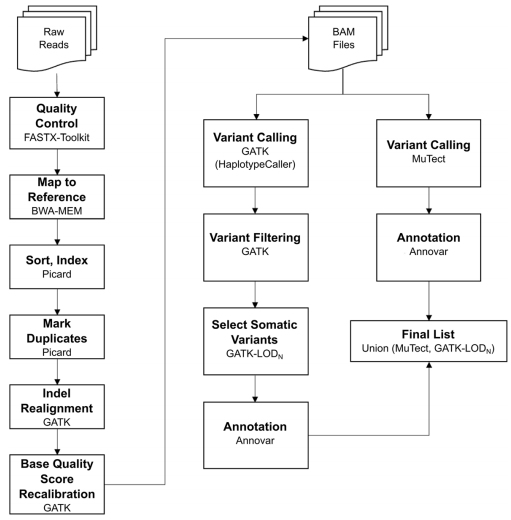
\includegraphics[scale=0.4]{GATK-LODn.png}
\caption{Workflow di GATK-LOD\ped{n}}
\label{fig: GATK-LODn}
\end{figure}

%\subsection{La statistica di base}

\subsubsection{GATK}
Il Genome Analysis Toolkit è un framework di programmazione creato da un gruppo di ricercatori di Boston, Massacchussets, assieme al Broad Institute di Harvard e l'MIT in Cambridge, Massacchussets, per facilitare lo sviluppo di programmi che analizzano l'enorme mole generati dal NGS, Next Generation DNA Sequencing \cite{McKenna2010}.
Infatti, l'utilizzo di questo sistema permette di sviluppare tools più solidi e performanti per il sequenziamento genetico.

La mancanza di strumenti flessibili e sofisticati dediti alla manipolazione dei dati di sequenziamento in maniera programmatica ha portato alla creazione di GATK.
Infatti, la maggior parte dei software che supportano l'analisi del DNA concedono alte prestazioni sono nella specifica area di interesse, senza mantenerle su differenti ambiti.
Questo deficit e l'emergere di un formato specifico per i prodotti del sequenziamento (SAM), hanno dato l'opportunità di ideare un software per la semplificazione delle analisi sui set di dati.

L'architettura di base per GATK è il MapReduce, il cui funzionamento implica la separazione delle computazioni in due passaggi.
Nel primo, l'intero problema è suddiviso in tanti elementi discreti indipendenti, i quali sono correlati alla funzione Map; nel secondo step, l'operatore Reduce riunisce gli esiti di Map in un unico risultato finale.
Siccome solo in certi casi, come la ricerca degli SNPs, vi è un adattamento naturale del sistema, GATK è costruito su traversals e walkers.
Le traversals sono schemi che provvedono alla preparazione e divisione dei dati; mentre le walkers consistono nei differenti moduli di analisi che computano i dati provenienti dalle prime.
Anche se GATK ha un numero ridotto di traversals, questo basta per soddisfare le esigenze della maggior parte della comunità di ricerca.
I due trasversal standard sono il "by each sequencer read" e il "by every read covering single base position in a genome", il cui uso è sfruttato per operazioni standard come la chiamata agli SNPs.
Il meccanismo di questi schemi non è riportato poichè non è stato ritenuto necessario per la comprensione di questo scritto.

Uno dei punti di forza dell'algoritmo è la capacità di gestire l'enorme quantità di materiale ricavato dal sequenziamento.
In particolare, GATK divide il tutto in pezzi chiamati "shard" che, al contrario della maggior parte dei sistemi di suddivisione, sono di una dimensione del multikilobase.
In questo modo non sono limitate le capacità della memoria e le prestazioni nel caso di parallelismo.
Questi shards contengono tutte le informazioni della regione genomica associata e sono trasmesse al trasversal prescelto.

Altre caratteristiche di GATK sono la possibilità di selezionare solo certe regioni del genoma, la parallelizzazione delle azioni da svolgere, l'organizzazione dei files di input grazie ad un'operazione di merging e la presenza di un walker relativo alla depth of coverage(DoC).

Il metodo stima il genotipo più probabile attraverso un semplice algoritmo Bayesiano, che ha funzione sia di punto di partenza per sviluppare nuovi classificatori; che di mettere in luce le capacità di parallelizzazione e di ottimizzazione della memoria disposte da GATK.
\'E importante sottolineare che è proprio la semplicità dell'operatore la causa di molti falsi positivi chiamati.

Il Genome Analysis Toolkit è quindi un framework che, grazie al suo nuovo approccio ai big data e alla piena libertà di sviluppo, fornisce strumenti importanti per l'elaborazione di algoritmi più specifici come il GATK-LOD\ped{n}.

\subsubsection{MuTect}
Il metodo MuTect è un algoritmo per la rilevazione delle mutazioni genomiche, che è stato creato per superare le scarse prestazioni dei meccanismi fino ad allora presenti \cite{Cibulskis2013}.
Infatti, quest'ultimi fornivano livelli di sensibilità e specificità considerati insoddisfacenti per una sufficiente comprensione delle anomalie.

Il sistema focalizza gli sforzi soprattutto sull'individuazione delle varianti a bassa frazione allelica, ovvero quelle regioni del DNA che originano e nutrono il tumore.
Queste frazioni sono tanto importanti quanto difficili da scovare poichè, mentre il meccanismo al loro interno determina il tipo di alterazione genomica, sia le regioni in cui si manifestano che la frequenza di occorrenza sono basse.

La conoscenza di questi tratti specifici favorisce lo studio sulle evoluzioni delle forme cancerogene e aiuta a proporre terapie di cura più affidabili.

L'esistenza di metodi a scarsa sensibilità e specificità ha quindi indotto un team di ricercatori dell'università di Boston, Massachussetts, assieme al Broad Insitute di Harvard e all'MIT in Cambridge, Massacchussets, a sviluppare il tool MuTect.
Questo strumento si è dimostrato sensibile e specifico nella scoperta degli eventi a bassa frequenza allelica, mantenendo alte prestazioni di specificità anche a frequenza superiori.

Nessuno dei modelli precedenti supporta tutti gli errori dei processi di sequenziamento ed è per questo che MuTect sfrutta due approcci di benchmarking per migliorare la performance: il downsampling e  i 'virtual tumors'.
Il primo misura la sensibilità con cui le mutazioni vengono chiamate, grazie a subset di dati con mutazioni già riconosciute.
Questo approccio è però limitato da alcuni aspetti che comprendono: il basso numero di eventi verificati, la sovrastima della sensibilità e l'impossibilità alla misurazione della specificità.
A causa dei limiti del downsampling è presente pure un secondo approccio, 'virtual tumors', che genera dei tumori virtuali conosciuti in ogni dettaglio.
I questa maniera i due metodi sono complementari e mentre il primo usa dati reali ma è limitato, il secondo è libero ma consuma materiale virtuale generato non perfettamente.
La sintesi dei due approcci permette di ricavare valori più veritieri della  sensibilità, misurare la specificità e colmare la maggior parte delle lacune derivate dal downsampling.

Previo allineamento ed esecuzione dei processi standard preanalisi, MuTect riceve i dati sequenziati sia dei campioni normali che dei cancerogeni, per poi eseguire quattro operazioni principali: la rimozione di dati a bassa qualità, la ricerca delle varianti, il filtraggio dei falsi positivi e la classificazione delle varianti.
La ricerca delle varianti consiste nell'applicazione di un primo metodo bayesiano, detto LOD\ped{T}, che adopera il rapporto tra due eventi probabilistici per determinare se è presente un variante.
Siccome il calcolo è condizionato da errori di sequenziamento, prima di ricavare la probabilità del variante è necessario applicare una serie di filtri che ne elimini la maggior parte, evitando così la sottostima dei falsi positivi.
Successivamente, si utilizza il secondo classificatore bayesiano LOD\ped{n}, implementato nel metodo GATK-LOD\ped{n}, per definire se il variante è somatico, germinale o indeterminato.

Gli esperimenti di verifica sulla sensibilità hanno evidenziato come MuTect sia uno strumento ad alto rilevamento soprattutto nelle mutazioni a frazioni alleliche basse.
Riguardo alla specificità sono due le fonti principali di falsi positivi: l'eccessiva chiamata a varianti, dovuta ad errori di sequenziamento, e la scarsa individuazione di eventi germinali, causato dalle insufficienti letture sul campione normale.
La gestione di tali errori è risolta con il miglior compromesso verificato tra sensibilità e specificità, che risulta nella scelta di mantenere alta la seconda a discapito della prima.

Complessivamente MuTect è un metodo che valorizza il compromesso tra il grado di rilevazione delle varianti e la loro corretta classificazione, producendo risultati affidabili.
In aggiunta, riporta sostanziali miglioramenti sulle analisi delle mutazioni a bassa frequenza allelica, la cui importanza è essenziale per le future ricerche biomediche.

\subsection{Il ruolo della fisica nella ricerca biomedica}
Nella prima metà del Novecento, dopo che l'introduzione della relativià di Einstein e la nascita della meccanica quantistica avevano ribaltato il pensiero della comunità scientifica, numerosi fisici si interessarono a problemi di biologia.
Il contributo fornito ad una così diversa area era sia di tipo matematico, dove la necessità di utilizzare equazioni e formule continuava ad aumentare nel corso degli anni, che di tipo teorica, ove l'uso di modelli già presenti nella fisica erano utili ad una comprensione più approfondita dei quesiti di biologia.
Il libro "What is life?" del fisico austriaco Erwin Schroedinger promosse il ruolo della fisica negli studi sull'ereditarietà a tal punto che gli scienziati Watson e Crick, che svelarono la struttura del DNA, lo accreditarono nelle loro pubblicazioni \cite{2058-7058-12-9-22}.
In seguito, numerosi fisici hanno contributo alla nascita della biologia molecolare e questa branca ha continuato a beneficiare della fisica sia per interpretare i problemi sotto un'ottica diversa, che per la confidenza che i fisici hanno riguardo alla modellizzazione dei sistemi complessi.
Difatti, la richezza della fisica nel saper gestire tali sistemi, l'elasticità nell'ampliare le proprie conoscenze a differenti campi di studio, insieme ad un approccio critico ma propositivo, si è rivelata un ingriedente necessario per il progresso della materia \cite{Pooley2005}.

Al passare del tempo e con il crescere delle ricerche, soprattutto nel campo biomedico, la presenza della fisica ha acquistato importanza sia nel ramo sperimentale che in quello teorico.
Nel primo, difatti, per anni le tecniche della cristallografia e della risonanza magnetica sono stati essenziali per i biologi molecolari, e, tuttora, le innovative tecniche della NGS concentrano gli sforzi su scovare quelle differenze proprietà fisiche che permettono di stabilire più velocemente i nucleotidi \cite{Zwolak2008}.
Nel secondo, invece, la fisica coopera con i bioinformatici sia nell'individuazione di modelli efficaci con cui affrontare i big data provenienti dai laboratori, che per l'analisi delle sequenze di DNA, sfruttando metodi provenienti esattamente dalla fisica statistica.

Nello specifico, la maggioranza dei modelli utilizzati e studiati sono basati sulla teoria dei network, la quale è stata ha acquisito uno spessore essenziale negli studi di biologia e di medicina.

\subsubsection{Teoria sui network}
La teoria dei network è materia prevalentemente dei fisici, dove per network si intende uno schema a base matematica che mira a rappresentare un sistema complesso, cercando di modellizzare le caratteristiche collettive. 
Un network è composto da elementi chiamati nodi, i quali sono collegati tramite percorsi, detti path, e tra cui sono presenti relazioni, denominate link. 
La teoria dei network è stata adottata e sviluppata per spiegare quelle leggi della natura di carattere generico e che hanno origine da manifestazioni stocastiche.
Gli strumenti matematici adoperati in questa teoria sono prevalentemente le matrici e i grafi, le cui proprietà garantiscono la massima espressione di connettività e di evoluzione che contraddinguono i sistemi complessi. 

I sistemi presenti in biologia sono generalmente un insieme di oggetti fortemente interagenti di cui si conoscono le proprietà; come possono essere ad esempio le reti geniche o il sistema nervoso umano.
Sono proprio i meccanismi dei network infatti la causa per cui non è più indispensabile ricostruire il codice genetico puntualmente, dato che risulta conveniente ricombinare tante stringhe casuali dello stesso filamento di DNA(shotgun sequencing).
Questa novità è ciò che contraddistingue il metodo Sanger dalle nuove tecniche del NGS e che permette a quest'ultime di ricavare i genomi di un individuo in tempi decisamente più ristretti.

La ricostruzione del genoma avviene, in particolare, a partire dal tutte le possibili sovrapposizioni dei frammenti sperimentali estratti. 
La scelta riguardo al ruolo dei frammenti e delle sovrapposizioni, ovvero stabilire chi è nodo e chi è link, è ciò che determina la teoria dei network da perseguire.
Il caso in cui i primi fossero i nodi e le seconde i link condurrebbe all'utilizzo di un path Hamiltoniano, cioè un percorso dove tutti i nodi vengono usati una volta sola.
All'opposto si avrebbe un path Euleriano, dove ogni link deve essere processato una singola volta e dove il problema è identificato dal grafo di De Brujin.
La differenza più netta tra i due path è la crescita di complessità, visto che il primo ha andamento non polinomiale mentre il secondo lineare, ed è da ciò che si valutano le capacità computazionali.

In conclusione, la teoria dei network unita all'utilizzo di macchine server performanti ha accelerato lo sviluppo di meccanismi sempre più raffinati per la ricostruzione del DNA, superando l'esaminazione prolungata in laboratorio con l'applicazione di congetture di fisica statistica.    

\section{Lo strumento di sviluppo: Snakemake}
\label{sec:SM}
Snakemake è un sistema di gestione del flusso di lavoro che semplifica l'esecuzione di algoritmi particolarmente complessi grazie all'utilizzo di un ambiente di sviluppo nitido ed intuitivo \cite{Koster2012}.
In più, questo software è specializzato nella scalabilità dei lavori, da singoli core fino all'uso di cluster, le cui transizioni non implicano pesanti modifiche al procedimento del sistema.

Questo programma è basato sul linguaggio di programmazione Python e la sua formazione è fortemente influenzata dal noto tool Make del sistema operativo Linux.
Ciò significa che Snakemake è modellato su una strategia di tipo \textit{pull} proprio come Make.
In un procedimento che segue la strategia \textit{pull}, ogni lavoro coinvolto comunica le proprie condizioni e la sequenza di esecuzione è determinata a partire dal richieste finali(modello \textit{"a valle"}).
Al contrario, la strategia \textit{push} esegue un procedimento a partire dai contenuti iniziali, attivando i compiti successivi una volta terminate le operazioni(modello \textit{"a monte"}). 

Il contenitore del codice Python in Snakemake è chiamato di default \textit{Snakefile} e l'ordine di esecuzione predefinito da linea di comando è:
\begin{lstlisting}
$ snakemake
\end{lstlisting}
Il sistema è strutturato, come Make, da un insieme di regole che rappresentano i compiti da svolgere nell'algoritmo, dove ognuna di esse contiene le tre informazioni fondamentali: input, output e azione.
\begin{lstlisting}[language=Python]
rule 'nome':
	input:

	output:

	shell/run/script:

\end{lstlisting}
Come si può vedere dal codice riportato, l'operazione avviene etichettando la regola con un certo 'nome' e inserendone all'interno le keyword \textit{input}, \textit{output} ed una tra \textit{shell}, \textit{run} e \textit{script}.
Rispettivamente le tre chiavi implicano l'utilizzo di comandi da terminale, l'esecuzione di un codice Python e l'avvio di uno script esterno.
La dichiarazione dei file di input e di output esprime le condizioni iniziali per la regola e il risultato atteso, così permettendo al programma di riconoscere le relative dipendenze e stabilire l'ordine di successione dei singoli lavori.
Per facilitare la comprensione del codice, è possibile creare, grazie al comando \textit{dot} della libreria Graphviz, un diagramma che schematizzi la sequenza delle regole.
Infatti questa sequenza, che ha il nome di \textit{DAG} (Directed Acyclic Graph), è visualizzata da \textit{dot} in una struttura ramificata dove i lavori sono rappresentati da nodi e dove le dipendenze sono semplicemente descritte da linee congiungenti. 
Dalla forma assunta da tale struttura è facile osservare che il lavoro degli sviluppatori del DAG è stato basato sulla teoria dei network e che l'applicazione di questa consente una descrizione semplice e compatta del sistema. 
L'utilità della schematizzazione consente anche di studiare quali dei lavori da eseguire sono parallelizzabili e quali, invece, devono mantenere una prestabilita sequenzialità. 
Ciò è possibile proprio dal fatto che il comando \textit{dot} rappresenta la successione delle regole solo e unicamente in base alle dipendenze reciproche, mantenendo quindi, ad esempio, la ripetizione di alcune regole sullo stesso livello di operatività.
Questo sistema di riconoscimento dei lavori potenzialmente simultanei da un contributo importante per impostare meccanismi di parallelizzazione. 

A proposito della gestione tecnica dei lavori, Snakemake ha un certo numero di proprietà che consentono di selezionare le caratteristiche computazionali desiderati. 
Due tra le funzionalità più rilevanti sono \textit{resources} e \textit{cores} che stabiliscono, da linea di comando, rispettivamente quali risorse delle macchine sono a disposizione e quanti core sono fruibili.
Le risorse possono includere ad esempio delle direzioni sulla gpu o sulla memoria accessibile (opzione \textit{mem}), mentre il numero di cores è essenziale per gestire i threads.

I threads sono fondamentali per un'esecuzione simultanea e il loro utilizzo avviene inserendo l'attributo \textit{threads} nel dominio di una regola.
L'assegnazione di un determinato numero di threads è comunque influenzato da un'eventuale opzione sui cores, dato che il numero di threads non può eccedere il numero di cores utilizzabili.
In particolare, oltre ai threads, è possibile specificare singolarmente per ogni regola anche le risorse disponibili, aggiungendo la voce \textit{resources} nel dominio. 

Altre due notevoli proprietà di Snakemake sono la portabilità e un innovativo meccanismo di inferenza.
La prima manifesta le poche dipendenze di installazione, dato che è in generale sufficiente dotarsi di Python; mentre la seconda rappresenta un moderno supporto all'inferenza per nome che si compie grazie a wildcards nominate nelle regole.

Le wildcards consistono in nomi che agiscono come parametri e che servono ad automatizzare le operazioni di riconoscimento delle dipendenze tra regole. 
In dettaglio, quando una variabile è associata ad una wildcard, è naturale che questa sia associata a più valori e che, quindi, il nome della variabile sia semplicemente una chiave. 
In presenza di una wildcard nell'input di una regola, i valori in essa contenuti sono ricercati negli output delle altre regole e, dopo aver tracciato le dipendenze, tale regola è eseguita una volta per ogni valore attribuito alla chiave.
Così agendo, le ripetizioni delle regole su diversi valori della wildcard sono sullo stesso piano di esecuzione, favorendo la parallelizzazione dei lavori.   
  

Una peculiarietà particolarmente utile di Snakemake è la capacità di riprendere l'esecuzione di una pipeline interrotta, esattamente dalla regola in cui si trovava al momento dell'interruzione.
Ciò è garantito dal fatto che il sistema attiva una regola solo se è assente il relativo output e, quindi, solo coloro che non sono state ultimate , o rimaste intoccate, prendono parte alla nuova esecuzione senza ripartire dall'inizio.
Chiaramente, questo approccio è modificabile richiendo esplicitamente che alla richiesta di una nuova istanza vengano sovrascritti i file di output e quindi acconsentita una diversa realizzazione.

Nella pipeline creata nell'ambito di questa ricerca, sono stati implementati altri attributi forniti da Snakemake.
Infatti, eccetto le chiavi di base, esistono diverse funzionalità che arrischiscono l'impostazione e la realizzazione delle regole, tra cui \textit{params}, \textit{threads}, \textit{benchmark} e \textit{conda}.
I primi due contengono rispettivamente i parametri indispensabili introdotti nell'azione e il numero di threads su cui l'azione può essere eseguita.
Quest'ultima proprietà richiama ad uno tra gli aspetti più importanti che hanno determinato la scelta di Snakemake, ovvero la capacità di gestire l'esecuzione della pipeline sulle risorse tecniche dei nodi di calcolo adoperati.
Le istruzioni sul numero di core da utilizzare, il numero di threads e la quantità di memoria da mettere a disposizione consentono di ricavare le configurazioni più efficienti, il tutto a beneficio dello sviluppo di metodi più potenti e ottimizzati.

A differenza delle prime due direttive, \textit{benchmark} e \textit{conda} richiedono una trattatazione più ampia.

In seguito alla spiegazioni di questi, è necessario dedicare un breve accenno ai file di configurazione spesso affiancati agli Snakefile.

\subsubsection{benchmark}
\label{subsubsec: SMb}
Quando è utilizzata la direttiva \textit{benchmark} in una regola, Snakemake trascrive su un file di testo i dettagli tecnici dell'operazione svolta.

Per primi sono riportati il tempo impiegato dal nodo per completare la regola sia in secondi che in ore, minuti e secondi.

A seguire, dal terzo al sesto sono mostrate le informazioni sull'uso della memoria.
In particolare:
\begin{itemize}
\item max\verb!_!rss è la massima memoria fisica non scambiata, che il processo usa(Resident Set Size);
\item max\verb!_!vms è la massima quantità totale di memoria virtuale utilizzata(Virtual Memory Size);
\item max\verb!_!uss è il massimo di memoria affidata unicamente al singolo lavoro, che esso impiega(Unique Set Size);
\item max\verb!_!pss è il massimo della quantità condivisa tra tutti i processi, che la regola sfrutta(Proportional Set Size).
\end{itemize}
Riguardo agli ultimi tre dettagli, sono presenti io\verb!_!in e io\verb!_!out che identificano le caratteristiche di input e output del processo; e mean\verb!_!load che descrive il carico medio sulla CPU.

\subsubsection{Conda}
Conda è una piattaforma per la gestione di svariati pacchetti ed è un pratico amministratore degli ambienti di elaborazione.
La cooperazione tra Snakemake e Conda, che avviene, come mostrato nel codice sottostante, inserendo la direttiva \textit{conda} nel dominio, favorisce un uso più flessibile degli ambienti.
\begin{lstlisting}
	conda:
		"path/to/directory/config_file.yaml"
\end{lstlisting}
Difatti, prima che lo Snakefile sia eseguito, Snakemake riconosce la voce \textit{conda} nella regola e richiama Conda per la creazione o attivazione dell'ambiente su cui essa sarà completata.
Le informazioni sull'ambiente da formare, nel caso esso debba essere creato, sono procurate da un file di configurazione indicato nel dominio ed è proprio questo che consente a Conda di generare l'ambiente e dotarlo dei requisiti richiesti.
Una volta che Conda ha terminato la creazione, l'ambiente è attivato e comincia l'esecuzione.
Chiaramente, questa fase di creazione avviene alla prima richiesta di un ambiente con determinate caratteristiche, così da procedere semplicemente con l'attivazione nelle successive computazioni.

Una tale opzione non costringe altri utilizzatori ad impostare manualmente l'ambiente principale come voluto dallo Snakefile, dato che ne sarà creato un apposito per la regola, e ciò ne alleggerisce l'utilizzo.
In aggiunta, questo meccanismo rende plastica la realizzazione del codice, vista la possibilità di dotare ogni regola di un proprio ambiente.


\subsection{I file di configurazione in Snakemake}
I file di configurazione sono oggetti, solitamente in formato yaml, dedicati alle istruzioni sui parametri contenuti nei codici principali.
Il ruolo di tali file è stabilire il valore delle chiavi che rappresentano i parametri.
Ad esempio, nel caso di Snakemake, un tipico file di configurazione ha forma: \verb! chiave: 'valore'!.
Il valore può essere un numero, una parola, un percorso o un file, ed esso rimane costante se non modificato direttamente nel codice sorgente o da linea di comando.
 Nell'ambito di Snakemake, il file di configurazione deve essere citato inizialmente con la linea \verb!configfile:'config_file.yaml'! e l'associazione tra chiavi e parametri è conseguita inizializzando una variabile secondo la seguente modalità.
\begin{lstlisting}[language=Python]
parametro = configfile['chiave']
\end{lstlisting}
I valori dei parametri possono essere modificati da terminale nel comando di avvio dello Snakefile, grazie all'argomento \textit{--config} seguito da una nuova inizializzazione, ad esempio \verb!chiave='nuovo_valore'!.

Il file di configurazione che si indica nella direttiva \textit{conda} ha, invece, una composizione differente, come mostrato nel codice riportato.
\begin{lstlisting}[language=Python]
channels:
  - esempio_canale
dependencies:
 -  esempio_dipendenza
\end{lstlisting}
Il dominio \textit{channels} determina su quale canale Conda deve lavorare, mentre \textit{dependencies} specifica quali pacchetti devono essere installati nell'ambiente.
In questo modo, dopo che Conda è chiamato da Snakemake per l'attivazione del particolare ambiente, esso controlla se ne è già presente uno con tali proprietà e, se esistente, lo attiva o, al contrario, prima lo istanzia.

Il contenuto dei file di configurazione è, in conclusione, determinante per il corretto, oltre che miglior, funzionamento del sistema.

\section{Le macchine low power e i nodi utilizzati}
\label{sec:LP}
I gruppi di ricerca che insistono nel proporre metodi avanzati per l'analisi dei big data in campo biomedico, non si limitano ad ottimizzare la sola componente software, bensì affrontano pure la scelta del tipo di componente hardware da adoperare.
Lo sviluppo di applicazioni sempre più raffinate ha richiesto infatti, nel corso del tempo, un progresso tecnologico che procedesse di pari passo e che permettesse di soddisfare in maniera esaustiva le richieste dei ricercatori.
Normalmente, i macchinari prediletti sono quelli più potenti e performanti che, pur essendo abili nel terminare i lavori previsti, hanno il difetto principale di consumare massicce quantità di energia.

Il dispendio di energia di uno strumento elettrico avviene, in particolare, alla conversione da corrente analogica (AC) a corrente digitale (DC): questo passaggio implica un'innalzamento della temperatura che causa lo sprigionamento di calore nell'ambiente circostante, da cui si ha una perdita di lavoro.
Tale effetto equivale ad uno spreco di energia ed esso si riproduce in ogni macchinario elettrico.
Il contenimento del calore, e quindi in generale una diminuzione dello spreco energetico, consente non solo una diminuzione dei costi per il sostentamento delle macchine, che può penalizzare le grandi aziende, ma anche il miglioramento della resa del nodo.
Difatti, il contenimento del calore implica la presenza di sistemi di raffreddamento che consumano grandi quantità di energia.
Un dato significativo relativo alle spese di raffreddamento è ad esempio sostenuto dal data center del INFN-CNAF(Centro nazionale delle tecnologie informatiche dell'INFN) a Bologna, dove il costo annuale per l'energia elettrica è dell'ordine del milione di euro.

L'altro difetto predominante è il costo che le macchine server tradizionali richiedono, che è dell'ordine delle migliaia di euro.

In aggiunta, un altro fattore penalizzante è dato dalla mancanza di scalabilità per aggiornare queste macchine, visto che ciò consisterebbe nell'acquisto di un'altra macchina più evoluta. 
Per i nodi low power invece, l'aggiornamento è facilmente accessibile.

Tali aspetti negativi hanno spinto vari team di studiosi ad interessarsi a differenti risorse computazionali, tra cui quella relativa alle macchine low power.
I macchinari low power sono strumenti che mirano ad abbassare il consumo energetico e soprattutto ad incrementare l'efficienza.

Questi strumenti, però, non sono una vera novità nel campo tecnologico, dato che alcuni oggetti, come gli orologi, possono essere già considerati tali.
La vera innovazione è l'impiego di strumenti di questo calibro nei processi computazionali sui big data.
Ovviamente, la differenza di performance tra i nodi low power e i macchinari utilizzati normalmente è netta, poichè tipicamente le prime hanno una potenza inferiore ai 45\,W(TDP).
Nonostante ciò, la cooperazione fra diversi nodi di tale genere, il cluster, potrebbe ambire a sostituire le macchine server moderne.
Questa tesi descrive proprio una ricerca introduttiva ad una questione così rilevante, che, difatti, considera la computazione non sul cluster ma solo su alcuni dei nodi a disposizione.

Le macchine server low power coinvolte in questa tesi sono state scelte con caratteristiche tecniche differenti, in modo da evidenziare fra talune una progressiva crescita delle prestazioni.
In più, è stata considerata anche una macchina tradizionale per poter comparare le diverse esecuzioni.

In accordo con il centro nazionale per la ricerca e lo sviluppo sulle tecnologie per l'informazione e la comunicazione (CNAF) dell'Istituto Nazionale di Fisica Nucleare, avente sede a Bologna, sono state utilizzate alcuni server ospitati al dipartimento di Fisica(figura \ref{fig:Cluster}).

\begin{figure}[H]
\centering
\subfloat[][\emph{Cluster Xeon D-1540 e Atom C2750.}]
	{\label{subfig:low_power}
	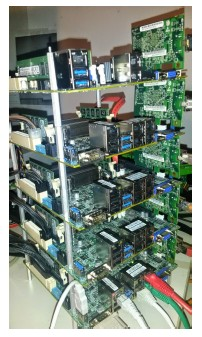
\includegraphics[scale=.5]{Avoton_Xeond.jpg}
	} \quad
\subfloat[][\emph{Cluster contenente bio8.}]
	{\label{subfig:bio8}
	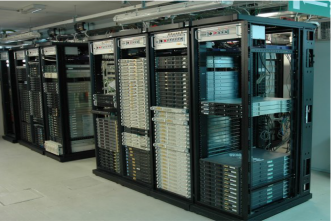
\includegraphics[width=.46\textwidth]{bio8.png}
	} \\
\caption{}
\label{fig:Cluster}
\end{figure}

I dettagli sui nodi dei cluster utilizzati per le computazioni sono esposti nelle tabelle sottostanti \ref{tab:cluster_generali} e \ref{tab:cpu}, che includono sia i tre nodi low power che un nodo di un server tradizionale (bio8).
In particolare, tutti i nodi montano processori con architettura X86\_64 su sistema operativo Linux Debian 9.

\begin{table}[H]
\begin{threeparttable}
\resizebox{1.0\textwidth}{!}{%
$\begin{array}{*{6}{c}}
	\toprule
		Nodo & CPU & Memory & Storage & Costo\text{*} & Consumo\text{*}  \\
	\midrule
		xeond & \text{1x Xeon D-1540} & 16\,GB & 8 TB(HDD) & \text{\euro 1000} & 60W\\
		avoton & \text{1x Atom C2750}  & 16\,GB & 5 TB(HDD) & \text{\euro 600} & 30W\\
		n3700 & \text{1x Pentium N3700}  & 8\,GB & 0.5 TB(SSD) & \text{\euro 130} & 8W \\
		bio8 & \text{2x Xeon E5-2620v4} & 12\,GB & 2 TB(HDD) & \text{\euro 10000} & 180W\\		
	\bottomrule
\end{array}$%
}
\begin{tablenotes}\footnotesize
\item[*] I valori di costo e consumo energetico sono stimati.
\end{tablenotes}
\end{threeparttable}
\caption{Caratteristiche dei nodi usati.}
\label{tab:cluster_generali}
\end{table}

\begin{table}[H]
\centering
\resizebox{1.0\textwidth}{!}{%
$\begin{array}{*{6}{c}}
	\toprule
		CPU & Microarchitecture(Platform)/litho & Freq(GHz) & Cores & Cache & TDP\\
	\midrule
		\text{Xeon D-1540} & Broadwell/14nm & 2.0(2.60) & 8(16) & 12MB & 45W \\
		\text{Atom C2750} & Silvermont(Avoton)/22nm & 2.40(2.60) & 8 & 4MB & 20W \\
		\text{Pentium N3700} & Airmont(Braswell)/14nm & 1.60(2.40) & 4 & 2MB & 6W \\
		\text{Xeon E5-2620v4} & Broadwell-EP/14nm & 2.10(3.00) & 8(16) & 20MB & 85W \\
	\bottomrule
\end{array}$%
}
\caption{Caratteristiche delle CPU dei nodi.}
\label{tab:cpu}
\end{table}

Si sottolinea che, in realtà, il nodo xeond appartiene ad un macchina con TDP pari a 45W e quindi è considerato al limite come macchina low power.

%Figura di GATK-LODn ?
%Figura che rappresenta gli step di GATK e MuTect?


\chapter{Procedimento}
Questo capitolo ha lo scopo di presentare il procedimento seguito per valutare l'ottimizzazione di una pipeline per l'analisi computazionale biofisica su nodi di cluster a basso consumo energetico.


In primo luogo sarà spiegato la componente principale creata per l'elaborazione, che implementa una parte del metodo GATK-LOD\ped{n}, e ne saranno approfonditi i singoli passaggi.

A seguire, saranno specificate quali computazioni sono state svolte, spiegando i motivi che hanno spinto a considerare talune, e il tipo di operazioni statistiche effettuate per modellare il prodotto delle analisi.



\section{Struttura delle simulazioni}
Il procedimento seguito dal sistema è suddivisibile in tre fasi: installazione, esecuzione e configurazione.


La prima di queste, la fase di installazione, evidenzia quali sono i fattori che permettono all'esecuzione di avvenire senza problemi.


In seguito, con la fase di esecuzione, è chiarita la struttura fondamentale del procedimento, ovvero la parte relativa all'algoritmo di analisi genetica, ed è definita la successione dei diversi passaggi: dalle estrazioni dei subset di DNA, fino alla produzione e semplicazione dei dati generati dal metodo.


Infine, sono esposte, nella fase di configurazione, le modalità di impostazione del programma, così da garantire una corretta gestione dei parametri e delle istruzioni da trasmettere ad esso.


\subsection{Installazione}
Il passaggio iniziale consiste nel predisporre l'ambiente di lavoro soddisfacendo i requisiti indispensabili per una valida esecuzione.

Nella preparazione di questa tesi, è stato scritto uno script apposito per questa fase preliminare, denominato \textit{installer.sh}, in modo da rendere questo procedimento compatto e più rapido.
Infatti, aver a disposizione un unico file da eseguire consente di automatizzare l'installazione e di garantire una gestione semplificato nel caso si parallelizzasse l'esecuzione su diversi nodi.

Questo eseguibile, in più, può risultare utile per coloro che sono già in possesso dei requisiti ma che preferiscono evitare di mischiare diversi ambienti di lavoro.
Ciò perchè l'installer aggiunge al bash script \textit{.bashrc} il percorso della directory Miniconda prodotta nell'installazione, così da indurre l'utilizzo di quei tool, tra cui \textit{Conda} e \textit{Snakemake}, inclusi nella medesima cartella.


Le due prerogative più importanti coinvolgono l'installazione di \textit{Conda}, che è inevitabile per l'attivazione degli ambienti, e ovviamente quella di \textit{Snakemake} per l'avvio del programma.


In seguito, sono richieste alcune librerie per Python, pandas e matplotlib, che sono necessarie per una fase di semplificazione dei benchmark e per le future analisi statistiche.
In più, pur non avendo uno spessore di primo piano, sono essenziali i tool PyYAML e psutil, che colmano alcune lacune dei contenuti principali installati.


Dopo aver superato tali punti, è fondamentale equipaggiarsi del genoma umano di riferimento e dei dati genetici che si desiderano sequenziare.


In relazione al progetto ivi presentato, il genoma umano di riferimento è stato ottenuto via web dal sito ufficiale del IGSR(International Genome Sample Resource); mentre il campione di DNA esaminato è stato scaricato dal database pubblico DDBJ(DNA Data Bank of Japan).


Conclusi gli interventi preparatori, può essere avviata l'esecuzione del procedimento senza dover curare altri aspetti.


\subsection{Esecuzione}
La fase esecutiva comprende una serie di processi che si possono raggruppare in tre macro sezioni ben definite.
La prima di esse descrive il processo di estrazione dei sottogruppi, o subset, di sequenze di DNA che si sceglie analizzare.
La seconda presenta la pipeline per l'analisi del genoma e dichiara quali sono i prodotti attesi.
La terza racchiude un'operazione di riordinamento e di semplificazione di tali ultimi prodotti per agevolare le successive indagini statistiche.



\subsubsection{Estrazione}
\label{subsubsec: ext}
Gli oggetti delle analisi sono i subset genetici che si sceglie di estrarre dall'intero genoma del soggetto e per questo è lecito accennare a come avviene l'estrazione.

Il genoma del soggetto è solitamente contenuto in un file in formato di testo \textit{fastq} che contiene le sequenze di nucleotidi rilevate durante le analisi in laboratorio.
Spesso però, la rilevazione non è singola ma, come nel caso di questo progetto, duplice e, quindi, i dati del paziente sono suddivisi in due file fastq accoppiati.

Brevemente, ogni singola lettura contenuta nel fastq è descritta da quattro linee aventi i seguenti ruoli: la prima linea marca la sequenza, la seconda mostra la sequenza, la terza identifica il punteggio di qualità e la quarta riporta tale punteggio.


Nel lavoro inerente a questa tesi, è stato scritto uno script in Python(\textit{split.py}) che svolge l'operazione di estrazione e per il quale, senza entrare in dettagli tecnici, è sufficiente trasmettere da linea di comando gli estremi della sezione che si vuole ricavare; come indicato di seguito.
\begin{lstlisting}[language=Python]
$ python split.py {inizio} {fine}
\end{lstlisting}
Grazie all'inserimento degli estremi, il programma calcola il numero di reads desiderate, seleziona le linee corrispondenti(il quadruplo del numero di letture) e le trascrive in un nuovo file fastq.

Ai fini dello studio finale, la disposizione di sottogruppi sia con diversi numero di sequenze che in diverse regioni consente di analizzare nei particolari le proprietà di scalabilità delle computazioni.

Siccome il numero di letture contenute è enorme, ed essendo che ad ognuna corrispondono quattro linee, la dimensione del file fastq è di conseguenza molto grande; per questo risulta funzionale dotarsi di un meccanismo per l'estrazione di sottogruppi.

La creazione di un unico programma anche per l'estrazione dei subsets conferma l'impegno nel dotarsi di un sistema automatizzato che possa elaborare pressochè senza interventi esterni.


\subsubsection{Algoritmo di ricostruzione genetica}
Una volta creati i subsets, può essere applicata la pipeline di ricostruzione genetica, che è interamente contenuta nell'apposito Snakefile.
\'E importante notare che la procedura seguita è ripresa dal metodo GATK-LOD\ped{n} solamente in alcuni passaggi.
Tali passaggi, in particolare, sono concretizzati nello Snakefile da regole che si susseguono l'un l'altra in base alle dipendenze di ciascuna(sezione \ref{sec:SM}).

L'algoritmo GATK-LOD\ped{n} è stato integrato solo fino al riallineamento di GATK, escludendo quindi i passaggi di riallineamento Indel e di ricalibrazione dei punteggi di qualità.
Allo stesso tempo non sono state considerate le fasi fondamentali di chiamata alle varianti e l'implementazione del classificatore LOD\ped{n} di MuTect, vera novità del metodo GATK-LOD\ped{n}.

Questa forte selezione degli step è stata voluta appositamente per non appesantire lo studio sull'ottimizzazione computazionale e, quindi, è stato scelto di concentrare le analisi solo su quelle operazioni che formano le basi dell'algoritmo per l'indagine del DNA.
In tale maniera, è facilitato sia l'indagine sulla scalabilità che il confronto tra i diversi nodi adoperati, così da poter trarre rapidamente le prime conclusioni.

I primi step consistono nell'indicizzazione del genoma umano di riferimento per i software che partecipano al sequenziamento.
Questi coinvolgono il software di allineamento BWA, il tool di manipolazione Picard, il gestore di strumenti Samtools e i programmi affini a GATK.
Per le prime tre  applicazioni, questa operazione è portata avanti da una specifica opzione delle stesse, mentre per l'ultimo essa è inclusa già nell'uso di Samtools.

Terminate le indicizzazioni, è sfruttato BWA MEM per la mappatura del DNA del soggetto sul genoma di riferimento che, inoltre, produce un file di etichetta, in formato \textit{SAM}, che è sottoposto ad un riordinamento da parte Picard con l'assistenza della modalità SortSam.

Dopo essersi procurati i file \verb!sorted_bam!, è eseguito il comando MarkDuplicates di Picard per identificare le letture doppie ed è generato un nuovo file \verb!dedup_bam!.
Elaborando quest'ultimo, la regola successiva crea un indice(in un file \textit{bai}) per il file \textit{bam} in modo da velocizzare l'analisi dei dati nel \textit{bam}; ciò è realizzato da un'altra funzionalità di Picard chiamata BuildBamIndex.

Per concludere, supportati dalla direttiva RealignerTargetCreator, propria del pacchetto GATK, il contenuto del file \textit{bam} è riallineato localmente in modo da diminuire ed evidenzire il numero di variazioni presenti.

Per riassumere l'intero processo è possibile osservare la raffigurazione seguente.
\begin{figure}[H]
\centering
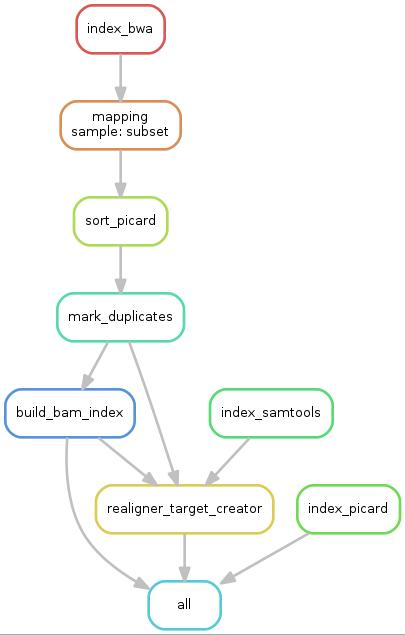
\includegraphics[scale=0.5]{Workflow.jpg}
\caption{Schematizzazione del procedimento implementato nella pipeline.}
\label{fig:workflow}
\end{figure}




\subsubsection{Organizzazione dei prodotti}
Il materiale su cui sono condotte le analisi statistiche sono i particolari tecnici e tempistici di ognuna delle regole completate.
Tali dati sono procurati, come già spiegato nella sezione \ref{subsubsec: SMb}, dalla direttiva benchmark in ogni passaggio.
Ciò significa che al termine dell'algoritmo sono prodotti tanti singoli file di benchmarking quante regole sono state completate, contando pure il caso in cui esse venissero ripetute ricorsivamente.
Per controllare la quantità di file e agevolare il futuro studio statistico, è stato scritto uno script in Python, denominato \verb!script_benchmark!.


Ogni file benchmark è dotato di un nome con funzione di etichetta; in particolare, la forma è la seguente.
\begin{lstlisting}[basicstyle=\fontsize{9}{6}\selectfont,breaklines=true]
benchmark_{name}_subset_{sample}_n_sim_{n_sim}_cputype_{cpu_type}_thrs_{thrs}_ncpu{n_cpu}.txt
\end{lstlisting}
Gli attributi contenuti nel nome indicano ordinatamente: il nome della regola completata, il tipo di campione analizzato, il numero della simulazione, il tipo di cpu utilizzata e il numero di threads e di cpu adoperati.
Mentre i primi due sono ricavati in automatico, gli altri fanno riferimento al file di configurazione dello Snakefile, come sarà spiegato nel paragrafo seguente.

Il lavoro svolto dallo script consiste quindi nel leggere ognuno dei file benchmark generati, considerare le etichette delle simulazioni e trasferire i dati incolonnati in un'unica tabella.
La tabella risultante non è dotata, quindi, solo delle colonne predefinite da \textit{Snakemake} nell'operazione di benchmarking(\ref{subsubsec: SMb}), bensì è arricchita dai dettagli contenuti nell'etichettatura.
In particolare, i dati sono organizzati nella tabella in ordine crescente rispetto al numero di simulazione.

All'avvio di questo script è controllato se è presente una tabella con lo stesso nome: in caso affermativo, i nuovi dati sono accodati ai precedenti; al contrario, ne è inizializzata un'altra.
In particolare, è necessario accedere al codice sorgente dello script se si vuole modificare il nome della tabella.

Attraverso questo sistema, il prodotto finale della fase di esecuzione, ed un unico oggetto dell'analisi statistica, è una tabella che racchiude le proprietà relative alle simulazioni ultimate.


Prima di procedere con l'esposizione dello studio effettuato su tali tabelle, è indispensabile perfezionare la descrizione del procedimento, specificando le opzioni di configurazione su cui essa si struttura.


\subsection{Configurazione}
Le ultime componenti del procedimento da delineare sono le modalità che definiscono le condizioni sotto cui deve essere portata avanti la computazione.
Queste componenti sono riportate nei file di configurazione e, per questa tesi, sono stati scritti due file di questo tipo che corrispondono rispettivamente a \textit{Snakemake} e a \textit{Conda}.

Le informazioni necessarie allo Snakefile sono procurate dal file \textit{config.yaml}, il quale comunica a \textit{Snakemake} alcuni dettagli della simulazione e le indicazioni su certe dipendenze.


Gli attributi della simulazione completano semplicemente l'etichettatura dei file di benchmarking e, pur rivestendo uno ruolo marginale, tali etichette permettono allo script di organizzazione dei dati una lettura rapida e quindi un'istanza immediata della tabella.
Come già citato precedentemente, i dettagli trascritti nel file di configurazione sono il tipo di cpu sfruttata, il numero della simulazione, il numero di threads adoperati e il numero di cpu coinvolte.

\'E stato scelto di gestire queste informazioni come parametri per non irrigidire il programma, visto che le macchine e i meccanismi usati possono essere innumerevoli.
Nello specifico, per modificare questi dettagli nelle etichette è sufficiente agire da linea di comando, come indicato nel paragrafo 1.2.1.

Sempre nello stesso file di configurazione sono presenti alcune chiavi che rappresentato le dipendenze non implementabili automaticamente negli ambienti di \textit{Conda} per \textit{Snakemake}.
Innanzitutto, sono presenti due indicazioni necessarie per il meccanismo di mapping, che sono l'utilizzo di \textit{Illumina} come piattaforma e di \textit{WES-Nextera-Rapid-Capture} come libreria.
A seguire, è indicato l'indirizzo in cui si può trovare il Genome Analysis ToolKit, da applicare nella procedura di riallineamento.

Altre istruzioni sulla configurazione del procedimento sono richieste da \textit{Conda} per la creazione, attivazione e disattivazione degli ambienti di lavoro durante l'esecuzione di \textit{Snakemake}(paragrafo 1.2.1).

Sempre nell'ambito di questa tesi, è stato scritto solo un documento di configurazione relativo a \textit{Conda}, dato che la maggior parte dei processi necessita di un ambiente con le stesse caratteristiche.
Nello specifico, quest'unico file di riferimento è contenuto nella directory \textit{envs} ed è chiamato \verb!config_conda.yaml!.

I requisiti richiesti per l'ambiente sono soddisfatti istruendo espressamente \textit{Conda} all'utilizzo del canale \textit{bioconda} per procedere con l'installazione di tre software coinvolti nel sequenziamento: \textit{BWA}, \textit{Picard} e \textit{Samtools}.

Ora che la natura del sistema è stata argomentata e sono stati approfonditi pure le procedure configurative, è possibile illustrare il percorso di studio statistico effettuato, accompagnato da una presentazione del genere di simulazioni conseguite.

\section{Studio statistico}
Questa sezione si occupa di descrivere quale tipologia di studio statistico è stato compiuto e quali sono state le simulazioni sostenute. 
In particolare, saranno indicate quali caratteristiche sono state considerate e quali relazioni sono state oggetto di studio.     

L'analisi dei dati è stata condotta utilizzando il linguaggio di Python \cite{Python}, sulla piattaforma iPython \cite{IPython}, e dotandosi delle librerie: Pandas \cite{pandas}, Matplotlib \cite{Matplotlib}, Seaborn \cite{seaborn}, NumPy \cite{Numpy} e SciPy \cite{Scipy}.

Il trattamento dei dati ha coinvolto inizialmente le funzioni sui dataframe di pandas per l'estrazione e la modifica delle tabelle finali ricavate al termine del procedimento.
Tali tabelle sono state ridotte ad un unico dataframe a cui sono state aggiunte quattro colonne per facilitare l'analisi. 
Le prime due contengono gli estremi del subset, ovvero la posizione della lettura iniziale e la posizione di quella finale, la terza contiene il numero di letture di ogni subset e la quarta il logaritmo del tempo di esecuzione.
Da questo unico contenitore sono state estratte progressivamente le tabelle utili alle varie analisi.

Il capitolo è suddiviso in tre sezioni, dove le prime due corrispondono alle caratteristiche principali su cui è stata condotta l'indagine statistica: il tempo di esecuzione e la memoria impiegata. 
L'ultima sezione include una semplice presentazione sul tipo di simulazioni che sono state completate.


\subsection{Analisi sul tempo di esecuzione}
\label{sbsec:Te}
Lo studio sul tempo di esecuzione è stato eseguito con lo scopo di delineare un andamento preciso di esso per ogni regola e per ognuna dei nodi adoperati.  

Inizialmente è stata derivata dal dataframe generale una tabella in cui ogni lavoro svolto corrispondesse a un subset e che quindi, non fossero presenti quelle regole indipendenti dal tipo di dati analizzati.
I lavori che dipendono dai dati sono, in ordine di esecuzione: la mappatura(mapping), l'ordinamento tramite picard(sort picard), la rilevazione dei duplicati(mark duplicates), la creazione dei file bam(build bam) e il riallineamento(realigner).
Al contrario, i processi indipendenti sono le indicizzazioni dello human reference per bwa, per picard e per samtools(index bwa, index picard e index samtools). 

In seguito è stata rappresentata su di un grafico la dipendenza del tempo di esecuzione di ogni regola rispetto alla grandezza del subset, identificando sullo questo stesso grafico un andamento per ogni nodo. 
In questa maniera è stato possibile verificare le differenze di prestazione tra le macchine server, adattando a ciascuna di esse la relazione matematica più idonea tra il tempo e il numero di sequenze del subset.

Una volta osservato l'andamento del tempo per ogni singola regola, l'attenzione è stata rivolta al tempo totale impiegato dalle regole dipendenti dal subset.
Per calcolare il tempo totale è stata creata una nuova tabella che contenesse tali regole, il tipo di cpu, il numero della simulazione e il tempo totale di esecuzione.

Un tale grafico consente di osservare come cresce il tempo di esecuzione complessivo all'aumentare del numero di letture e come ciò è influenzato dal tipo di macchina adoperata.

Terminato lo studio sui lavori dipendenti dalla grandezza dei subset, sono state brevemente considerate anche le regole indipendenti.
Anche in questo caso è stata tracciata su un grafico la dipendenza del tempo di esecuzione rispetto ad ogni regola, distinguendo il comportamento tra i differenti nodi.  

Infine, sono stati estratti subset di ugual grandezza ma con letture differenti, che sono stati messi in relazione con le durate delle singole regole rispetto.
Così operando, è possibile osservare se il tempo di completamento dei lavori è influenzato dal contenuto del subset processato e con quale entità ciò influisce.

Il tempo impiegato per concludere ogni regola non è però l'unico fattore da prendere in considerazione, visto che per promuovere l'uso della parallelizzazione è indispensabile analizzare le modalità di utilizzo della memoria. 

\subsection{Analisi sulla memoria fisica}
\label{subsec:Mf}
La memoria fisica studiata è ottenuta grazie a Snakemake dal tool psutil sottoforma di una memoria detta RSS o \textit{Resident Set Size}(paragrafo \ref{subsubsec: SMb}). 
In realtà, l'unica operazione conseguita da Snakemake è prelevare le informazioni in bytes su questo tipo di memoria e convertirlo in MB per l'utente.
Perciò nel corso della spiegazione, la memoria trattata si riferisce proprio a questa informazione trasmessa da Snakemake.  

I dettagli sulla memoria che viene impiegata nei singoli processi è di fondamentale importanza per un corretto sviluppo di un futuro sistema parallelizzato.
Infatti, lo studio sull'andamento di tale memoria consente di verificare fino a che livello di scalabilità la cpu è proficua e quando il suo uso comincia a saturare.
Questi comportamenti indicano fino a che punto è possibile ottimizzare l'utilizzo dei core della cpu e identificano le memorie richieste dai vari lavori.
Distinguere quali sono i processi che necessitano maggiormente di memoria e quelli che ne utilizzano una scarsa percentuale, permette di conoscere quali sono i nodi per le varie regole che ottimizzano l'esecuzione.

Lo studio statistico condotto è stato interessato, come per le tempistiche, ad osservare il comportamento della memoria in base alle regole, ai subsets e ai diversi nodi.
Perciò, è stata inizialmente posta in relazione la memoria occupata da ogni regola con il numero di sequenze del subset, distinguendo le macchine.
Successivamente è stata eseguita la stessa operazione per le regole indipendenti dai dati ed infine, è stato studiato il comportamento della memoria lasciando invariato il numero di letture ma considerandone diverse.
È stato trascurata, invece, la somma delle memoria in ogni passaggio perchè non sono ritenute informazioni da cui trarre beneficio. 
    

%\subsection{Analisi sui processi di input ed output} 
%Due ulteriori dati che Snakemake trascrive nel benchmark sono ottenuti da psutil, specificatamente dalla funzione \verb!disk_io_counters!, e sono il numero di bytes letti e quelli scritti dal processo.
%In particolare, questi sono rispettivamente nominati \verb!io_in! e \verb!io_out! e, come per la memoria rss, sono convertiti in megabytes da Snakemake. 
%
%Queste due proprietà garantiscono una conoscenza più approfondita di come la cpu partecipa alla computazione, evidenziando con quale intensità, espressa in MB, essa è coinvolta nelle distinte operazioni.
%Così come l'analisi di rss, la statistica sulle fasi di input ed output delinea gli effetti che i lavori causano sul nodo.
%Da queste informazioni si può trarre una valutazione su quanto al massimo è possibile servirsi della cpu e fino a che punto l'utilizzo di essa è efficace.
%
%Le analisi realizzate sono state le stesse che per la memoria rss e quindi sono stati studiati gli andamenti dell'input e dell'output per le regole dipendenti dai subset e pure quelle indipendenti.
%Ugualmente ai casi precedenti sono state valutate anche le dipendenze per il tipo di cpu e sono stati confrontati intervalli diversi aventi identico numero di letture.
%Non è stato presa in esame il valore complessivo per l'input e output nell'intero arco dell'esecuzione perchè da tale dato totale non è possibile ricavare alcuna informazione proficua.
 
\subsection{Le simulazioni completate} 
\label{subsec:simc}
Le simulazioni che sono state eseguite ai fini di questa tesi sono state scelte per valutare le performance sui nodi dei cluster a disposizione, in modo da evidenziarne la potenziale scalabilità.

I nodi low power adoperati, che sono stati illustrati nel paragrafo \ref{sec:LP}, sono stati impiegati in base alle loro diverse potenze computazionali e sono stati confrontati con un nodo del cluster bio8, utilizzato come riferimento per le macchine tradizionali.
È stato utilizzato un solo core per ognuno dei nodi in tutto l'arco del procedimento, rimandando ad un futuro sviluppo l'utilizzo del multicore.  


Tutti i nodi hanno processato gli stessi subset di dati con un numero di letture iniziale pari a 5000 fino a 3 milioni, passando per i multipli di diecimila, di centomila e di un milione.
In questo modo è stato possibile studiare le potenzialità delle macchine a processare dati identici con larghezza crescente e come questo incremento condiziona l'uso della cpu. 

Solamente sui nodi xeond e bio8 sono state portate avanti le simulazioni fino a subset con un numero di letture pari a 9 milioni, continuando da 3 milioni a scalare progressivamente di 1 milione.

Non sono stati fatti proseguire anche gli altri nodi perchè lo scopo della tesi è valutare il comportamento dei nodi su piccoli subset di dati e quali indicazioni questo possa dare per sviluppare un'esecuzione parallelizzata efficace.
Visto che per tale valutazione sono stati sufficienti i dati citati, solo le due macchine più performanti sono andati oltre per confermare le stime ottenute.

Ciò significa che tutte le simulazioni sono state svolte solamente su una piccola frazione delle letture in possesso. 
Infatti il numero di letture complessivo del paziente era ben oltre i 45 milioni e la massima grandezza di un subset condivisa tra tutti i dispositivi è stata di 3 milioni, che equivale circa al $6.7\%$.
Per xeond e bio8 invece, i subset sono stati allargati in prossimità del $20\%$.

In dettaglio, queste simulazioni sono state ripetute dieci volte per i nodi xeond e bio8 mentre sono bastate cinque volte per gli altri nodi, dato che i tempi di completamento del processo arrivavano già a coprire un arco di tempo considerevole.

Infine utilizzando lo script \verb!split.py! descritto nella sezione \ref{subsubsec: ext}, sono stati estratti subsets contenenti letture diverse, ma dello stesso numero, che sono stati studiati in una fasie delle analisi.
L'unico numero di letture considerato è stato centomila e ciò è stato eseguito solo per i nodi dei cluster low power, e quindi non da bio8.

Nel capitolo seguente saranno esposti gli esiti più rilevanti, selezionati dai prodotti finali dell'analisi statistica effettuata sui dati delle simulazioni.  


\chapter{Risultati}
\label{cap:3}
I risultati finali sono stati suddivisi nelle due caratteristiche su cui è stata sviluppata l'analisi dei dati.
Sono quindi presenti una sezione relativa ai tempi di esecuzione e una sulla memoria fisica sfruttata. 
La descrizione delle relazioni più interessanti è, inoltre, accompagnata dall'utilizzo di alcuni tra i grafici elaborati durante lo studio statistico.

In sede di analisi sono stati usati subset con dimensione minima di centomila.

\section{Tempi di esecuzione}
L'indagine sui tempi di esecuzione, come spiegato nel paragrafo \ref{sbsec:Te}, è stata condotta approfondendo le seguenti relazioni: i tempi di esecuzione per le regole, la durata complessiva del processo e i tempi impiegati per intervalli differenti con lo stesso numero di sequenze. 
Questa sezione si occuperà di presentare gli esiti finali più rilevanti di ognuno di tali aspetti.

\subsection{Tempi e regole}
Le regole previste dal procedimento hanno concentrato l'analisi su due campi, una relativo a quei processi che non dipendono dal tipo di dati considerato e uno relativo a quelli che invece dipendono. 
Considerando le prime, è evidente dalla figura \ref{fig:Tind} come l'unico processo significativo sia l'indicizzazione dello human reference per BWA, mentre le rimanenti non influiscano in alcun modo. 
In più, la differenza tra le potenze computazionali è netta già da questa figura, dato che tra il nodo migliore e il peggiore vi è uno scarto di più di un'ora.
\begin{figure}[H]
\centering
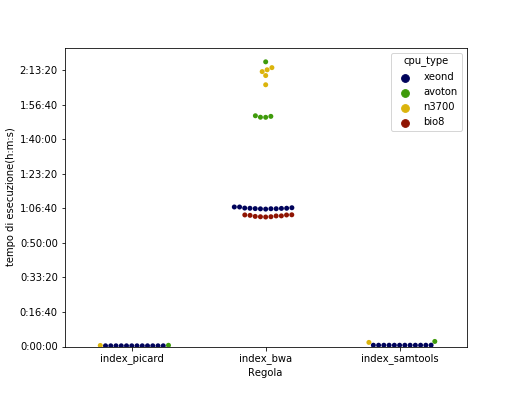
\includegraphics[scale=0.46]{Tind.png}
\caption{Tempi di esecuzione per le regole indipendenti dal subset.}
\label{fig:Tind}
\end{figure}
Nonostante la durata per l'indicizzazione sia notevole, questa fase è riprodotta una sola volta per tutti i successivi lavori, visto che è riferita solamente al genoma umano di riferimento.

Passando alle regole dipendenti, i grafici riportati nelle figure \ref{subfig:BB}, \ref{subfig:Map}, \ref{subfig:MD}, \ref{subfig:Rlg} e \ref{subfig:SP} mostrano i vari andamenti per la grandezza dei subset.

Per ciascuna figura viene anche riportata una tabella con i dettagli delle rigressioni lineari effetuate per descrivere il tempo di esecuzione in funzione del numero di sequenze lette.
La regressione è stata effettuata con il metodo di Theil-Sen.
Questo metodo implica una regressione lineare robusta, ovvero che non risente della presenza di outlayer nei dati.

Nelle tabelle viene riportato l'intervallo di confidenza della pendenza della retta.
Visto che nessuno di questi intervalli di confidenza contiene lo zero, per tutte le regole c'è una dipendenza significativa fra il numero di sequenze ed il tempo impiegato.

\begin{figure}[H]
\centering
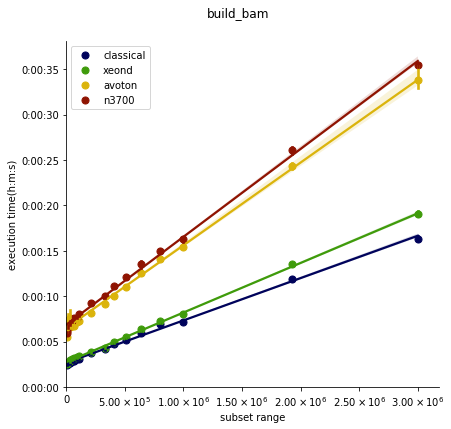
\includegraphics[scale=0.7]{build_bam.png}
\captionof{figure}{Tempi per Build BAM.}
\label{subfig:BB}
\end{figure}

\begin{table}[H]
    \centering
	\begin{tabular}{lrrrr}
	\toprule
	{} &         pendenza & intercetta &     min pendenza &     max pendenza \\
	\text{tipo di cpu} & $\frac{secondi}{\text{\num{e6} letture}}$ & $secondi$ & $\frac{secondi}{\text{\num{e6} letture}}$ & $\frac{secondi}{\text{\num{e6} letture}}$ \\
	\midrule
	avoton   & {9.2} &        6.4 &   {9} & {9.5} \\
	bio8     & {4.4} &        3.1 & {4.4} & {4.4} \\
	n3700    & {9.4} &        7.4 & {9.3} & {9.5} \\
	xeond    & {5.3} &          3 & {5.3} & {5.3} \\
	\bottomrule
	\end{tabular}
	\caption{Dettagli retta di fit per Build BAM.}
	\label{tab:Bb}
\end{table}

\begin{figure}[H]
\centering
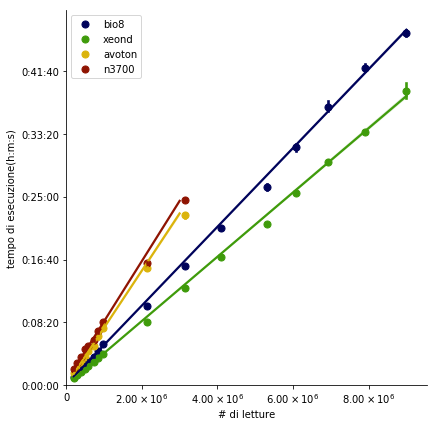
\includegraphics[scale=0.7]{mapping.png}	
\captionof{figure}{Tempi per Mapping.}
\label{subfig:Map}
\end{figure}

\begin{table}[H]
	\centering
	\begin{tabular}{lrrrr}
	\toprule
	{} &         pendenza & intercetta &     min pendenza &     max pendenza \\
	\text{tipo di cpu} & $\frac{secondi}{\text{\num{e6} letture}}$ & $secondi$ & $\frac{secondi}{\text{\num{e6} letture}}$ & $\frac{secondi}{\text{\num{e6} letture}}$ \\
	\midrule
	avoton   &{440} &        6.8 &{430} &{45} \\
	bio8     &{310} &        7.9 &{310} &{310} \\
	n3700    &{470} &         24 &{470} &{480} \\
	xeond    &{250} &       -3.3 &{250} &{250} \\
	\bottomrule
	\end{tabular}
    \caption{Dettagli retta di fit per Mapping.}
    \label{tab:Mp}
\end{table}

\begin{figure}[H]
\centering
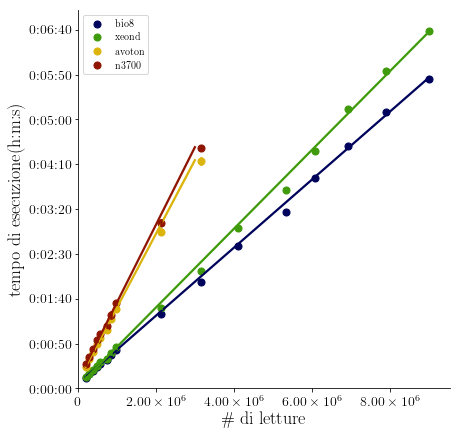
\includegraphics[scale=0.7]{mark_duplicates.png}
\captionof{figure}{Tempi per Mark Duplicates.}
\label{subfig:MD}
\end{figure}

\begin{table}[H]
    \centering    
	\begin{tabular}{lrrrr}
	\toprule
	{} &         pendenza & intercetta &     min pendenza &     max pendenza \\
	\text{tipo di cpu} & $\frac{secondi}{\text{\num{e6} letture}}$ & $secondi$ & $\frac{secondi}{\text{\num{e6} letture}}$ & $\frac{secondi}{\text{\num{e6} letture}}$ \\
	\midrule
	avoton   &{81} &        7.9 &{81} &{82} \\
	bio8     &{38} &        4.7 &{38} &{38} \\
	n3700    &{86} &        8.9 &{85} &{87} \\
	xeond    &{44} &        2.4 &{43} &{44} \\
	\bottomrule
	\end{tabular}
    \caption{Dettagli retta di fit per Mark Duplicates.}
	\label{tab:Md}
\end{table}

\begin{figure}[H]
\centering
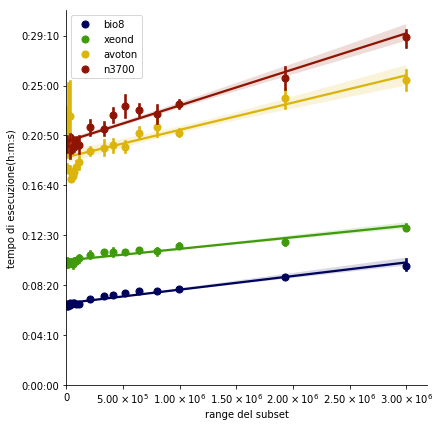
\includegraphics[scale=0.7]{realigner.png}
\captionof{figure}{Tempi per i tempi di Realigner.}
\label{subfig:Rlg}
\end{figure}

\begin{table}[H]
	\centering
	\begin{tabular}{lrrrr}
	\toprule
	{} &         pendenza & intercetta &     min pendenza &     max pendenza \\
	\text{tipo di cpu} & $\frac{secondi}{\text{\num{e6} letture}}$ & $secondi$ & $\frac{secondi}{\text{\num{e6} letture}}$ & $\frac{secondi}{\text{\num{e6} letture}}$ \\
	\midrule
	avoton   &{130} &    \num{1.2e+03} &{110} &{160} \\
	bio8     &{38} &    \num{4.5e+02} &{36} &{39} \\
	n3700    &{150} &    \num{1.3e+03} &{120} &{170} \\
	xeond    &{38} &    \num{6.8e+02} &{36} &  {40} \\
	\bottomrule
	\end{tabular}
    \caption{Dettagli retta di fit per Realigner.}
	\label{tab:Rlg}
\end{table}

\begin{figure}[H]
\centering
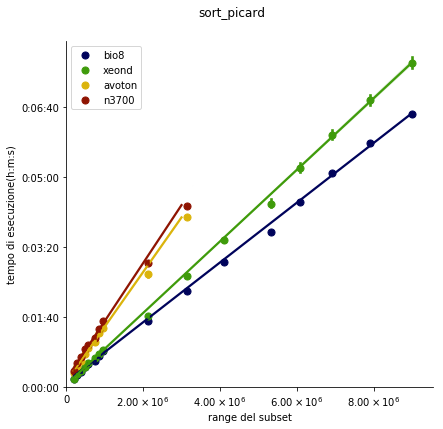
\includegraphics[scale=0.7]{sort_picard.png}
\captionof{figure}{Tempi per Sort Picard.}
\label{subfig:SP}
\end{figure}

\begin{table}[H]
    \centering
	\begin{tabular}{lrrrr}
	\toprule
	{} &         pendenza & intercetta &     min pendenza &     max pendenza \\
	\text{tipo di cpu} & $\frac{secondi}{\text{\text{\num{e6} letture}}}$ & $secondi$ & $\frac{secondi}{\text{\num{e6} letture}}$ & $\frac{secondi}{\text{\num{e6} letture}}$ \\			\midrule
	avoton   & 80 &        6.5 & 79 & 83 \\
	bio8     & 43 &        7.9 & 43 & 43 \\
	n3700    & 84 &         12 & 83 & 86 \\
	xeond    & 51 &        2.9 & 51 & 51 \\
	\bottomrule
	\end{tabular}
    \caption{Dettagli retta di fit per Sort Picard.}
    \label{tab:Sp}
\end{table}

L'unica regola che mostra una particolarità è la fase di riallineamento(realigner Figura \ref{subfig:Rlg}), in cui il tempo di avvio della regola, rappresentato dall'intercetta, costituisce una parte importante del tempo complessivo di esecuzione della regola stessa. 

Nei grafici sono distinguibili due gruppi di nodi significativamente confrontabili: avoton e n3700, xeond e bio8.
Questa distinzione è confermata dai valori delle pendenze riportate nelle tabelle \ref{tab:Bb}, \ref{tab:Md}, \ref{tab:Mp}, \ref{tab:Rlg} e \ref{tab:Sp}.
In particolare, il fatto che xeond e bio8 condividano lo stesso genere di architettura(tabella \ref{tab:cluster_generali}) indica come questa caratteristica possa influenzare l'esecuzione.

Infine, dai grafici si può notare che le regole di lunga durata sono il mapping e il realigner, mentre quella che impiega il minor tempo è il build bam.
Riguardo a mark duplicates e sort picard, si nota che queste regole condividono la stessa durata e la stessa crescita(tabelle \ref{tab:Md} e \ref{tab:Sp}).    


\subsection{Durata complessiva}
Un altro aspetto rilevato è stato il tempo complessivo richiesto per svolgere tutti i passaggi che esclusivamente dipendono dal numero di reads nel subset, escludendo tutti i passaggi non dipendenti (come l'indicizzazione del reference umano fatto da BWA).
Questi tempi sono rappresentativi del tempo richiesto per la pipeline per ciascun paziente. 

\begin{figure}[H]
\centering
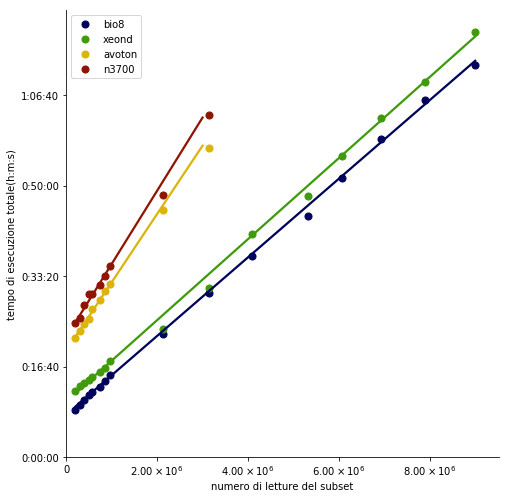
\includegraphics[scale=0.7]{Tempi_complessivi.png}	
\captionof{figure}{Tempi complessivo di esecuzione.}
\label{fig:Ttot}
\end{figure}

\begin{table}[H]
    \centering
	\begin{tabular}{lrrrr}
	\toprule
	{} &         pendenza &    intercetta &     min pendenza &     max pendenza \\
	\text{tipo di cpu} & $\frac{secondi}{\text{\num{e6} letture}}$ & $secondi$ & $\frac{secondi}{\text{\num{e6} letture}}$ & $\frac{secondi}{\text{\num{e6} letture}}$ \\
	\midrule
	avoton   &{760} & \num{1.2e+03} &{730} &{790} \\
	bio8     &{440} & \num{4.7e+02} &{440} &{440} \\
	n3700    & {800} & \num{1.3e+03} &{770} &{830} \\
	xeond    &{390} & \num{6.8e+02} &{390} & {400} \\
	\bottomrule
	\end{tabular}
    \caption{Pendenze per i tempi complessivi.}
    \label{tab:Ttot}
\end{table}

I grafici in figura \ref{fig:Ttot} e i valori in tabella \ref{tab:Ttot} confermano che i nodi sono separati in due coppie comparabili: avoton e n3700, xeond e bio8.


\subsection{Variabilità dei tempi di esecuzione}
Tutti i subset utilizzati nella sezione precedente condividono la stessa posizione iniziale di estrazione.
Per valutare la variabilità del tempo di esecuzione dalla posizione iniziale di estrazione, sono state ripetute le analisi con subset di stessa lunghezza ma con diversi punti di estrazione.
Questi punti di estrazione sono stati scelti in modo da non aver sovrapposizione fra questi subset e il numero di letture stabilito è stato centomila

\begin{table}[H]
\centering
\resizebox{1.0\textwidth}{!}{
\begin{tabular}{lrrrrr}
\toprule
regola & {build bam} & {mapping} & {mark duplicates} & {realigner} & {sort picard} \\
\text{tipo di cpu} &           &           &            &            &   \\
\midrule
avoton   &  $7.3\pm0.2$ &  $60\pm14$ & $16.4\pm0.3$ &  $1110\pm50$ &   $12.8\pm0.4$ \\
n3700    &  $8.00\pm0.18$ & $74\pm3$ & $18.4\pm0.8$ &  $1250\pm60$ &   $14.7\pm0.4$ \\
xeond    &  $3.27\pm0.07$ & $30\pm11$ &  $8.1\pm0.6$ &   $610\pm30$ &    $7.2\pm0.9$ \\
\bottomrule
\end{tabular}
}
\caption{Media e deviazione standard, espresse in secondi(s), dei tempi di esecuzione delle regole su diversi subset da centomila reads.}
\label{varT}
\end{table}

I dati associati a ciascuna regola indicano che i nodi tendenzialmente si stabilizzano su valori fissati.
Infatti, eccetto il mapping che mostra l'andamento meno stabile, i nodi impiegano la stessa quantità di tempo senza dipendere dal contenuto delle reads. 


\section{Memoria utilizzata}
La memoria occupata dai singoli processi è stata studiata analogamente al tempo trascurando però lo studio di una memoria complessiva per tutti i passaggi. 
Ciò implica che sono state analizzate in un primo momento le occupazioni della memoria per ognuna delle regole e poi è stato tentato di definire l'andamento per diversi intervalli con stesso numero di letture.
La memoria intesa in questo capitolo si riferisce alla memoria "Resident Set Size" ricavata dal tool psutil e riportata da Snakemake, come già indicato nel paragrafo \ref{subsec:Mf}. 

\subsection{Consumo di memoria per le regole}
Le informazioni sui vari comportamenti sono tratte dai grafici in figura \ref{fig:RSSr} e dalla tabella \ref{Tab:maxmem}.
\begin{figure}[H]
\centering
\subfloat[][\emph{Memoria utilizzata da Build BAM.}]
	{\label{subfig:BB_rss}
	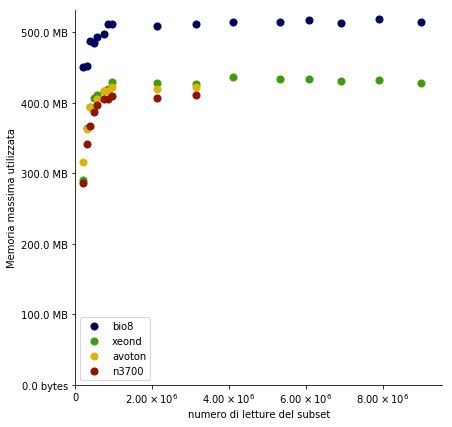
\includegraphics[width=.46\textwidth]{Max_rss_build_bam.png}
	} \quad
\subfloat[][\emph{Memoria utilizzata da Mapping.}]
	{\label{subfig:Map_rss}
	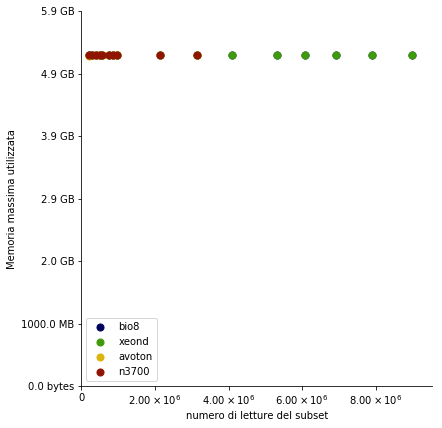
\includegraphics[width=.46\textwidth]{Max_rss_mapping.png}
	} \\
\end{figure}
\begin{figure}[H]
\ContinuedFloat
\centering
\subfloat[][\emph{Memoria utilizzata da Mark Duplicates.}]
	{\label{subfig:MD_rss}
	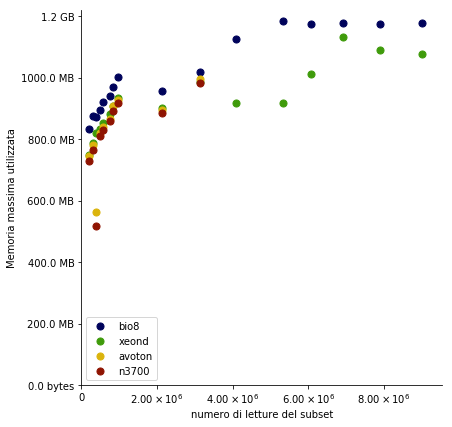
\includegraphics[width=.46\textwidth]{Max_rss_mark_duplicates.png}
	} \quad
\subfloat[][\emph{Memoria utilizzata da Realigner.}]
	{\label{subfig:Rlg_rss}
	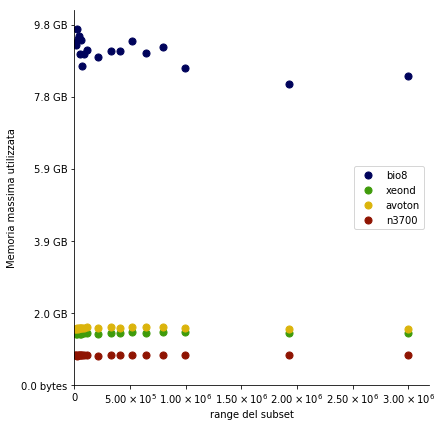
\includegraphics[width=.46\textwidth]{Max_rss_realigner.png}
	} \\
\end{figure}
\begin{figure}[H]
\ContinuedFloat
\centering
\subfloat[][\emph{Memoria utilizzata da Sort Picard.}]
	{\label{subfig:SP_rss}
	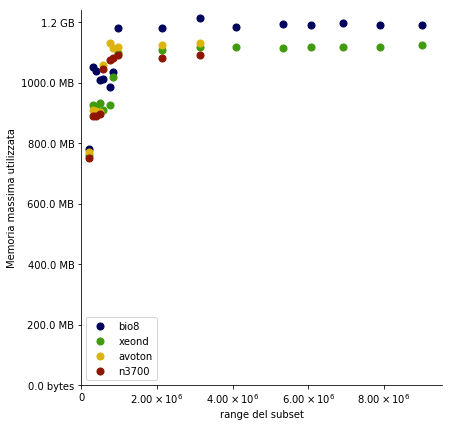
\includegraphics[width=.46\textwidth]{Max_rss_sort_picard.png}
	} 
\caption{}
\label{fig:RSSr}
\end{figure}

\begin{table}[H]
\centering
\begin{tabular}{lrrrrr}
\toprule
regola &  \text{build bam} &  mapping &  \text{mark duplicates} &  realigner &  \text{sort picard} \\
\text{cpu type} &            &          &                  &            &              \\
\midrule
avoton   &        429 &     5305 &             1019 &       1626 &         1150 \\
bio8     &        527 &     5295 &             1042 &      10362 &         1232 \\
n3700    &        419 &     5306 &              988 &        859 &         1115 \\
xeond    &        435 &     5305 &             1004 &       1582 &         1138 \\
\bottomrule
\end{tabular}
\caption{Tabella dei massimi valori di memoria impiegati, espressi in MB.}
\label{Tab:maxmem}
\end{table}


Si può vedere che nelle regole di marcamento dei duplicati(figura \ref{subfig:MD_rss}), di formazione del file BAM(figura \ref{subfig:BB_rss}) e di riordimento per picard(figura \ref{subfig:SP_rss}), la memoria satura superando il milione di reads. 

Le altre regole che analizzano specificatamente i dati, la mappatura(figura \ref{subfig:Map_rss}) e il riallineamento(figura \ref{subfig:Rlg_rss}), hanno entrambe un'occupazione fissa della memoria.
Nel caso del mapping, infatti, tutte le macchine occupano la stessa quantità di memoria, indicando una saturazione generale, mentre nel riallineamento ciascuna cpu utilizza una quantità fissata di memoria che sembra essere una frazione della memoria totale disponibile. 

Per le regole che non dipendono dal paziente, riportate in figura \ref{fig:RSSind}, la richiesta di memoria non sembra invece dipendere significativamente dal nodo.

\begin{figure}[H]
\centering
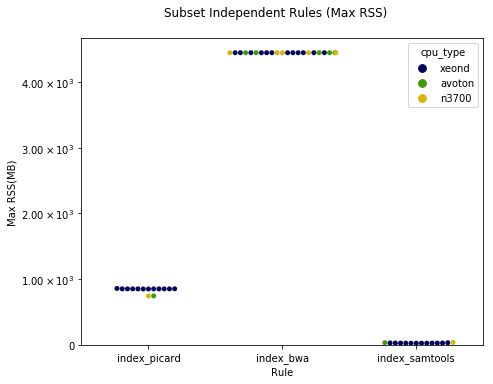
\includegraphics[scale=0.46]{Max_rss_ind.png}
\caption{Memoria impiegata dalle regole indipendenti dai subsets.}
\label{fig:RSSind}
\end{figure}

\subsection{Variabilità della memoria occupata}
Lo studio sulla memoria impiegata per intervalli diversi con ugual numero di sequenze è stato compiuto solo sui nodi dei cluster low power. 
La tabella \ref{varM} riporta la media e la deviazione standard per ciascuna regola, su ogni nodo.
In particolare il numero di reads considerato è stato di centomila.

\begin{table}[H]
\centering
\resizebox{1.0\textwidth}{!}{
\begin{tabular}{lrrrrrrrrrr}
\toprule
regola & {build bam} & {mapping} & {mark duplicates} & {realigner} & {sort picard} \\
\text{tipo di cpu} &             &            &              &            &                 &           &            &            &             &           \\
\midrule
avoton   &  $240\pm8$ &  $5279.0\pm0.7$ & $702\pm7$ &  $1600\pm15$ & $585\pm3$ \\
n3700    &  $222\pm4$ &  $5280\pm6$ &  $686\pm7$ &   $830\pm11$ & $572\pm3$ \\
xeond    &  $230\pm12$ &  $5280\pm16$ &  $703\pm6$ &  $1430\pm30$ & $576\pm3$ \\
\bottomrule
\end{tabular}
}
\caption{Media e deviazione standard, espresse in MB, della memoria occupata dalle regole su diversi subset da centomila reads.}
\label{varM}
\end{table}

I valori ottenuti evidenziano che la memoria è fortemente stabile in ogni regola, per ogni macchina.
Ciò conferma che le operazioni sfruttano la stessa quantità di memoria indipendentemente dal contenuto dei subset e, eccetto il caso del realigner, ne occupano pressochè lo stesso valore. 


%\section{Processi di I-O} 
%Gli ultimi risultati sono stati ottenuti dall'indagine sui processi di input e output coinvolti nel completamento di ogni lavoro.
%Questa sezione, sugli stessi modelli precedenti, è stata suddivisa in due parti che determinano come la lettura e la scrittura sono dipendenti dal set di dati e se il contenuto di tali dati incide sull'uso della macchina.
%
%\subsection{I-O e regole}
%Il primo esito riportato è per le regole indipendenti dai subset ed a parte l'indicizzazione per BWA l'impatto è praticamente nullo.
%\begin{figure}[H]
%\centering
%\subfloat[][\emph{Scrittura per regole indipendenti dai subset}]
%	{\label{subfig:Iind}
%	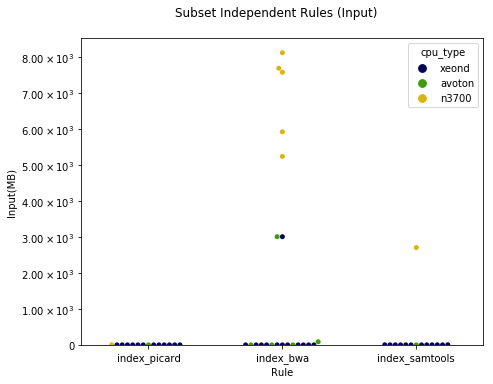
\includegraphics[width=.46\textwidth]{I_ind.png}
%	} \quad
%\subfloat[][\emph{Scrittura per regole indipendenti dai subset.}]
%	{\label{subfig:Oind}
%	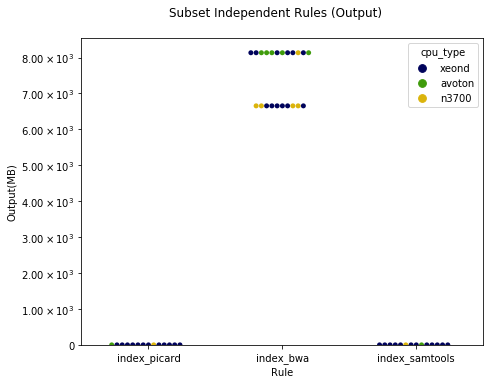
\includegraphics[width=.46\textwidth]{O_ind.png}
%	} \\
%\caption{}
%\label{fig:RSSrng}
%\end{figure}
%Diversamente dai tempi e dalla memoria, il lavoro di indicizzazione non è sempre costante sia per il caso di input che per quello dell'output.
%Riguardo all'input, le macchine più performanti (Xeon e Pentium N3700) nella maggior parte delle volte non eseguono alcuna lettura, mentre la rimanente varia in modo imprevedibile per valori elevati.
%Per l'output invece, l'andamento è costante per Pentium, al contrario di Xeon e Atom che similmente occupano due valori ben distinti. 
%
%
%Considerando le regole che invece dipendono dal subset, sono elecanti di seguito gli andamenti dei due processi per ognuna di esse.
%\begin{figure}[H]
%\centering
%\subfloat[][\emph{Lettura per la mappatura}]
%	{\label{subfig:IM}
%	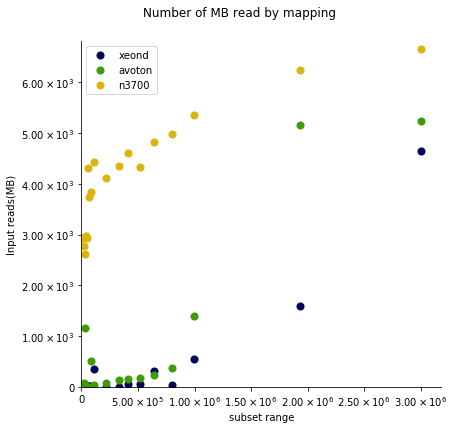
\includegraphics[width=.46\textwidth]{IO_Input_mapping.png}
%	} \quad
%\subfloat[][\emph{Scrittura per la mappatura}]
%	{\label{subfig:OM}
%	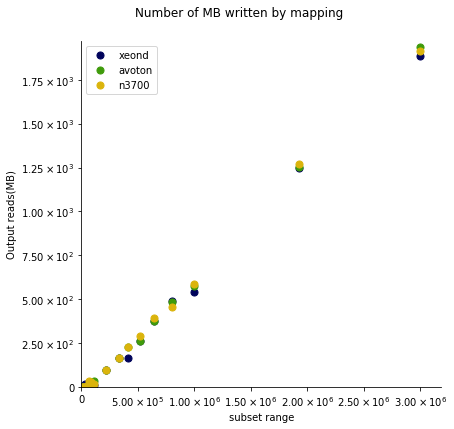
\includegraphics[width=.46\textwidth]{IO_Output_mapping.png}
%	} \\
%\caption{}
%\label{fig:IOm}
%\end{figure}
%
%La fase di lettura per la mappatura sembra crescere esponenzialmente per le due macchine migliori mentre per Pentium N3700 la crescita ha un andamento che tende a saturare in maniera logaritmica. 
%Gli elementi finali di Atom non seguono però un'esponenziale, suggerendo che avvenga una saturazione anche per le altre due macchine per grandezze dei subset superiori.
%
%La fase di scrittura, invece, mostra una andamento lineare praticamente omogeneo per tutte le macchine.  
%
%\begin{figure}[H]
%\centering
%\subfloat[][\emph{Lettura per il sorting di picard}]
%	{\label{subfig:ISp}
%	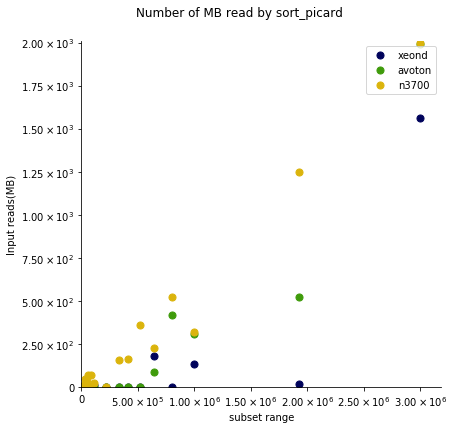
\includegraphics[width=.46\textwidth]{IO_Input_sort_picard.png}
%	} \quad
%\subfloat[][\emph{Scrittura per il sorting di picard}]
%	{\label{subfig:OSp}
%	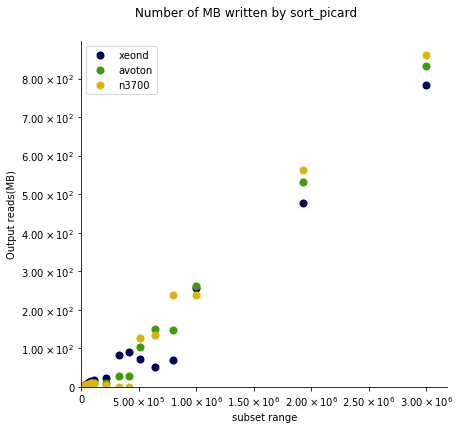
\includegraphics[width=.46\textwidth]{IO_Output_sort_picard.png}
%	} \\
%\caption{}
%\label{fig:IOSp}
%\end{figure}
%
%Per Picard il lavoro di riordinamento è ambiguo nella lettura perchè le macchine incrementano con traiettorie non ben definibili.
%Ad esempio, per Pentium la traiettoria potrebbe essere adattata ad una retta, ma esiste un certo sotto gruppo di dati che descrive una direzione nettamente diversa, così vanificando tale ipotesi.
%
%La scrittura invece inizia ad assumere contorni più chiari dopo una certa grandezza del subset, oltre il quale, tende a crescere linearmente. 
%Prima di raggiungere tale grandezza difatti ogni macchina, per numero di sequenze diversi, mostra un avvallamento non motivabile direttamente da questo tipo di studio statistico.  
%
%\begin{figure}[H]
%\centering
%\subfloat[][\emph{Lettura per la marcatura dei duplicati}]
%	{\label{subfig:IMd}
%	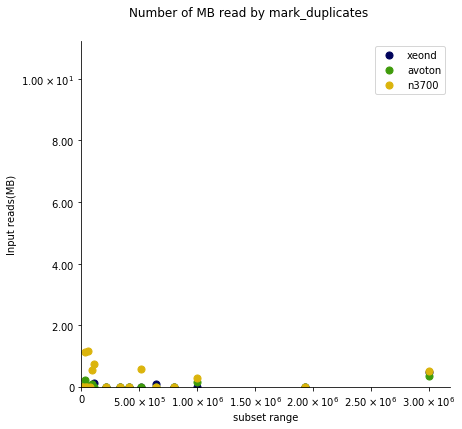
\includegraphics[width=.46\textwidth]{IO_Input_mark_duplicates.png}
%	} \quad
%\subfloat[][\emph{Scrittura per la marcatura dei duplicati}]
%	{\label{subfig:OMd}
%	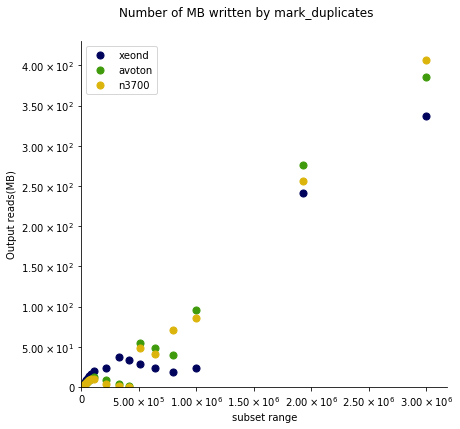
\includegraphics[width=.46\textwidth]{IO_Output_mark_duplicates.png}
%	} \\
%\caption{}
%\label{fig:IOMd}
%\end{figure}
%
%La descrizione della marcatura dei duplicati determina che la fase di lettura è coinvolta solo marginalmente, dato che esaurisce in generale meno di $2\,MB$, mentre quella di scrittura segue la stessa attitudine che il sorting per picard.
%Infatti ciò è evidente soprattutto in Xeon, per cui prima di avanzare con linearità è ben delineato un ventre di una curva.  
%
%\begin{figure}[H]
%\centering
%\subfloat[][\emph{Lettura per la formazione del BAM}]
%	{\label{subfig:IBB}
%	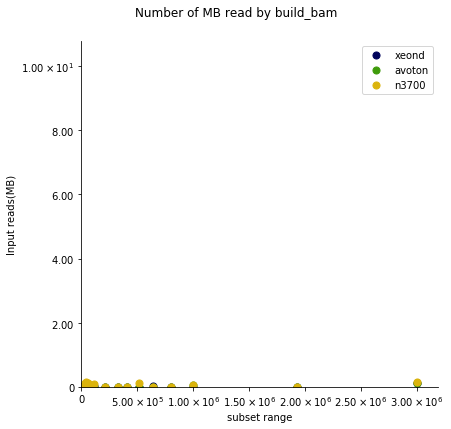
\includegraphics[width=.46\textwidth]{IO_Input_build_bam.png}
%	} \quad
%\subfloat[][\emph{Scrittura per la formazione del BAM}]
%	{\label{subfig:OBB}
%	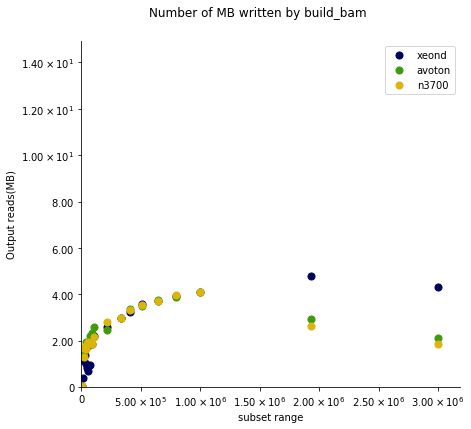
\includegraphics[width=.46\textwidth]{IO_Output_build_bam.png}
%	} \\
%\caption{}
%\label{fig:IOBB}
%\end{figure}
%
%Riguardo al passaggio per la costruzione dei file BAM, il numbero dei megabytes letti è trascurabile. 
%Al contrario, la scrittura segue una crescita logaritmica fino a circa 1 milione di subset, per poi cominciare a calare vistosamente.
%
%Le ragioni di questo calo non sono spiegabili, come nei casi precedenti, semplicemente osservando tale relazione dato che sarebbe più esauriente un approfindimento sia sulle prestazione dei macchinari che sul funzionamento dell'algoritmo di formazione del BAM. 
%
%\begin{figure}[H]
%\centering
%\subfloat[][\emph{Lettura per il riallineamento}]
%	{\label{subfig:IR}
%	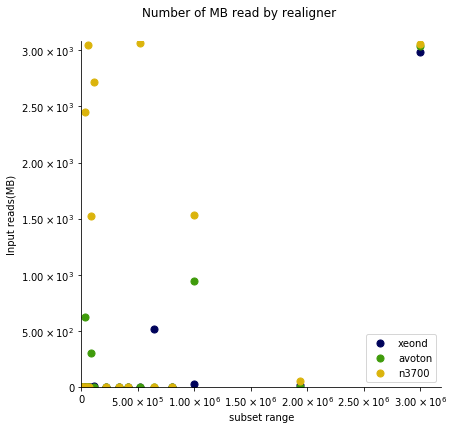
\includegraphics[width=.46\textwidth]{IO_Input_realigner.png}
%	} \quad
%\subfloat[][\emph{Scrittura per il riallineamento}]
%	{\label{subfig:OR}
%	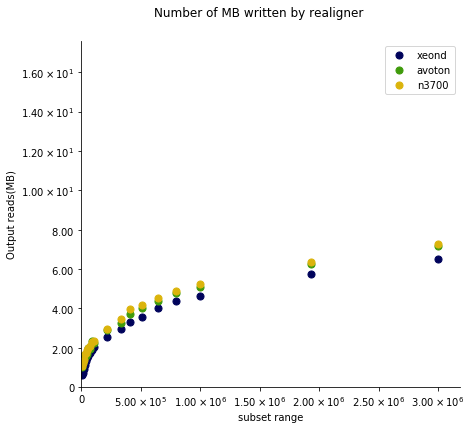
\includegraphics[width=.46\textwidth]{IO_Output_realigner.png}
%	} \\
%\caption{}
%\label{fig:IOR}
%\end{figure}
%
%In coda, il riallineamento mostra contemporaneamente il carattere meno comprensibile per la fase di lettura e quello più nitido per la fase di scrittura.
%I valori riportati nel grafico di input sono difficili da decifrare; non vi è un andamento univoco ne tra le cpu ne tra i dati associati ad ognuna di esse.
%Sono presenti un numero considerevole di processi che consumano una percentuale infinitesima in input che, però, sono alternati a salti elevati di letture, che tra loro non suggeriscono alcun andamento ben fissato.
%Evidentemente la natura del metodo di riallineamento influenza pesantemente questa fase di scansione dei bytes, riproducendo una lettura di essi fortemente discontinua.
%
%Nettamente diverso è il caso della scrittura, dove i dati tracciano una curva simile ad un logaritmo senza essere dotati di valori estranei ad essa.
%In più, i vari andamenti sono ordinati rispetto alla potenza computazionale delle macchine anche se, in questo frangente, con discrepanze molto sottili.
%
%\par Prima di passare al caso degli intervalli diversi con stesso intervallo, è utile sottolineare quali sono i lavori che generalemente consumano più bytes in fase di lettura e scrittura.
%In entrambi i casi è il mapping che vanta l'utilizzo maggiore e, all'opposto, è la formazione dei BAM che necessita del minor uso delle operazioni di input e output. 
%L'unico passaggio che presenta una netta inversione nell'uso di lettura e scrittura è, come si può controllare in figura \ref{fig:IOR}, il riallineamento, per cui sarà necessario uno studio specifico.
%
%\subsection{I-O per stessi range}
%L'ultima valutazione è stata eseguita, allo stesso modo che per i tempi e la memoria,  su intervalli diversi con lo stesso numero di letture.
%Sono stati scelti i grafici sottostanti per illustrare gli andamenti più interessanti ricavati durante le analisi.
%\begin{figure}[H]
%\centering
%\subfloat[][\emph{Input per realigner su range diecimila}]
%	{\label{subfig:IRdieci}
%	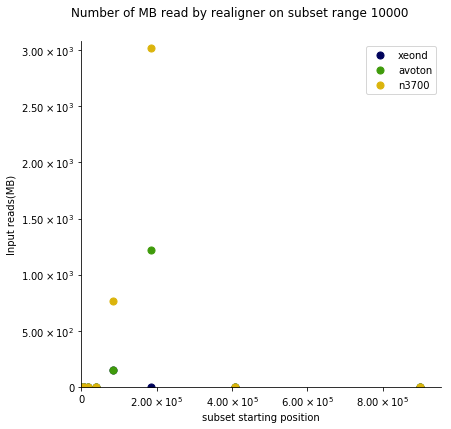
\includegraphics[width=.46\textwidth]{IO_I_realigner_dieci.png}
%	} \quad
%\subfloat[][\emph{Output per realigner su range diecimila}]
%	{\label{subfig:ORdieci}
%	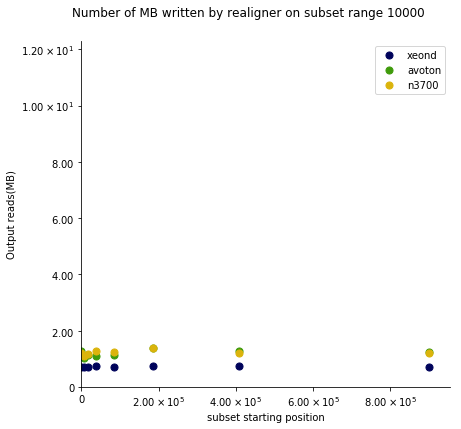
\includegraphics[width=.46\textwidth]{IO_O_realigner_dieci.png}
%	} \\
%\end{figure}
%\begin{figure}[H]
%\ContinuedFloat
%\centering
%\subfloat[][\emph{Input per mapping su range centomila}]
%	{\label{subfig:MIcento}
%	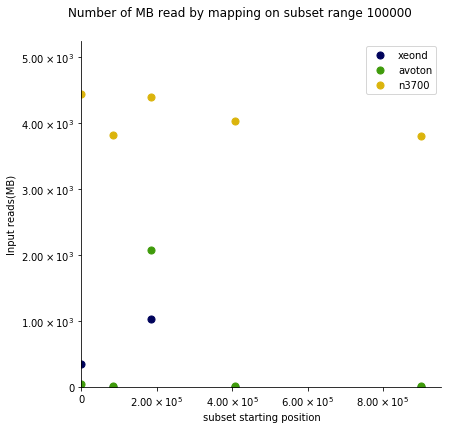
\includegraphics[width=.46\textwidth]{IO_I_map_cento.png}
%	} \quad
%\centering
%\subfloat[][\emph{Output per mapping su range centomila}]
%	{\label{subfig:MOcento}
%	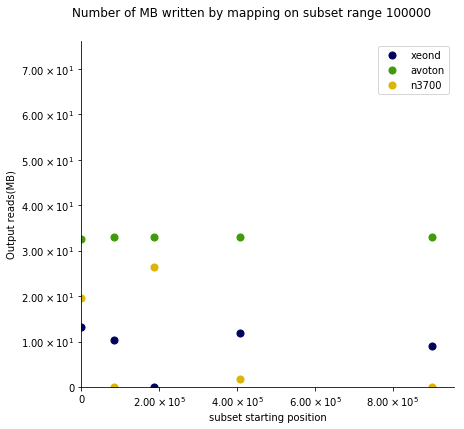
\includegraphics[width=.46\textwidth]{IO_O_map_cento.png}
%	} 
%\caption{}
%\label{fig:IOrng}
%\end{figure}
%
%I passaggi di scrittura mostrano un andamento più omogeneo per tipo di subset, pressochè costante nel caso della figura \ref{subfig:ORdieci} e per Atom(avoton) in \ref{subfig:ORdieci}.
%\'E interessante notare come le macchine computino con modalità diverse e che ciò causi la perdita dell'ordine delle cpu, dalla migliore alla peggiore, che caratterizzava le analisi per i tempi e la memoria.  
%
%Diverso è il caso della lettura che è rappresentato sia in \ref{subfig:IRdieci} che in \ref{subfig:MIcento}.  
%Le varie tracce non seguono andamenti ben definiti e sono spesso accompagnati da netti salti tra le misure di lettura, i quali inducono a pensare che sia il contenuto dei subset a determinare il tipo di lettura da svolgere. 

\chapter{Conclusioni}
I risultati esposti nel capitolo \ref{cap:3} sono le informazioni basilari per lo sviluppo futuro di una tecnica adeguata per la parallelizzazione dei processi.
Ciascuna caratteristica studiata mostra le potenzialità di un singolo nodo di un cluster definendone il singolo andamento e confrontandolo con gli altri presenti.

Tutte le analisi svolte sono state conseguite selezionando solamente una piccola frazione delle letture in possesso, spingendosi al massimo intorno al $6.7\%$. 
Infatti il numero di letture complessivo era ben oltre i 45 milioni e la massima grandezza di un subset condivisa tra tutti i dispositivi è stata di 3 milioni.

Solamente per il nodo più performante, con cpu Xeon, è stato deciso di spingersi oltre arrivando ai 9 milioni di letture contenute in un subset, che equivale a circa il $20\%$. 

Le conclusioni..

Questa tesi ha avuto lo scopo di riunire tutti gli elementi che hanno partecipato allo studio dell'analisi computazionale biofisica su nodi di macchine a basso consumo energetico, per preparare le basi ad un importante sviluppo futuro.  
Le prossime fasi che saranno coinvolte nella ricerca infatti, necessitano di un'iniziale analisi sui componenti computazionali più fondamentali perchè vengano fornite le informazioni per programmare una tecnologia efficace, fruibile ed economica.

Il percorso di studio futuro avrà come primo step il confronto dei dati con un modello di macchina tradizionale, non low power, tra quelle utilizzate quotidianamente.
In seguito saranno adattate le simulazioni all'utilizzo contemporaneo di tutti i core previsti dalle macchine, visto che solo uno step del procedimento è stato trattato con un core aggiuntivo(il mapping).
Infine le analisi verranno svolte, dopo un'opportuna progettazione, su un gruppo di cluster low power per verificare concretamente che l'utilizzo di un insieme cooperante di apparecchi a basso consumo energetico è effettivamente performante almeno quanto una macchina tradizionale.

L'esito positivo della ricerca consentirebbe agli enti accademici e ospedialieri di adottare una tecnologia più accessibile, meno costosa e soprattutto più veloce, che sostenga la ricerca in medicina e in biologia, oltre che il generale progresso scientifico.




\bibliography{Bib_Tesi}

\end{document}
